% VanniKawachh -- B.Tech thesis (v2 concept)
% Source: docs/THESIS.md. Constants and measured numbers transcribed exactly;
% no acoustic accuracy or hardware radio figures are claimed (Phase 1-2 WIP).
\documentclass[12pt,a4paper]{report}

\usepackage{amsmath}
\usepackage{amssymb}
\usepackage{graphicx}
\usepackage{booktabs}
\usepackage[margin=1in]{geometry}
\usepackage{setspace}
\usepackage{url}
\usepackage{hyperref}

\graphicspath{{../figures/v2/}{../figures/}}

\onehalfspacing
\setlength{\emergencystretch}{3em}
\tolerance=2000

\begin{document}

% ---------------------------------------------------------------- title page
\begin{titlepage}
\centering
{\LARGE\bfseries VanniKawachh: A Distributed AI Acoustic Intelligence
and Autonomous Drone Response Network for Women Safety\par}
\vspace{1.5cm}
{\large\bfseries A Thesis\par}
\vspace{0.5cm}
{\large Submitted in partial fulfilment of the requirements of the\\
Bachelor of Technology in Computer Science and Engineering\par}
\vspace{1cm}
{\large by\par}
\vspace{0.3cm}
{\large\bfseries Group CSE\_B\_04\par}
\vspace{0.5cm}
{\large Shivansh Verma \quad Saksham Sabadra \quad Rudra Thakur \quad
Rohan Untawale\par}
\vspace{1cm}
{\large under the guidance of\par}
\vspace{0.3cm}
{\large\bfseries Dr.~Aditya Turankar\par}
\vspace{1.5cm}
{\large Department of Computer Science and Engineering\\
G.~H.~Raisoni College of Engineering, Nagpur\par}
\vspace{0.5cm}
{\large\bfseries Session 2026--27\par}
\vfill
\end{titlepage}

% ---------------------------------------------------------------- certificate
\pagenumbering{roman}

\chapter*{Certificate}
\addcontentsline{toc}{chapter}{Certificate}

This is to certify that the thesis entitled \emph{``VanniKawachh: A
Distributed AI Acoustic Intelligence and Autonomous Drone Response
Network for Women Safety''}, submitted by Group CSE\_B\_04 --- Shivansh
Verma, Saksham Sabadra, Rudra Thakur, and Rohan Untawale --- in partial
fulfilment of the requirements of the Bachelor of Technology in
Computer Science and Engineering, is a record of work carried out by
the group under my guidance at the Department of Computer Science and
Engineering, G.~H.~Raisoni College of Engineering, Nagpur, during the
session 2026--27.

\vspace{2.5cm}
\noindent
\begin{tabular}{@{}p{0.45\textwidth}p{0.45\textwidth}@{}}
Dr.~Aditya Turankar & Head of Department \\
Guide & Department of Computer Science and Engineering \\
\end{tabular}

\vspace{1cm}
\noindent\emph{(Signatures, seal, and date --- to be completed.)}

% ---------------------------------------------------------------- declaration
\chapter*{Declaration}
\addcontentsline{toc}{chapter}{Declaration}

We declare that this thesis is our own work, carried out by us as
Group CSE\_B\_04 under the guidance of Dr.~Aditya Turankar, and that
all sources of material used --- software libraries, protocol
specifications, model checkpoints, regulatory texts, and surveyed
literature --- are cited in the References. The software described
herein is published under the repository
\url{https://github.com/SV-1411/drone.git}, and all experimental
results reported are reproducible from that repository as described in
Chapter~\ref{ch:testing}. A large-language-model assistant was used
during drafting for structure and consistency; all technical content
derives from the implementation and its test logs, and every sentence
was reviewed and accepted by the authors.

\vspace{1.5cm}
\noindent\emph{(Signatures, date --- to be completed.)}

% ---------------------------------------------------------------- abstract
\chapter*{Abstract}
\addcontentsline{toc}{chapter}{Abstract}

Crimes against women concentrate where help is hardest to summon: dark
streets, forest stretches, campus outskirts, parking areas --- places
that are simultaneously camera-poor, patrol-poor, and often cellular
dead zones. The safety technology deployed against this problem almost
universally burdens the victim: panic-button apps, wearables, and
carried devices all presume a charged, reachable, operable device in
the victim's hand at the worst moment of her life. This thesis
designs, implements, and validates \textbf{VanniKawachh}
(``voice-shield''), a system that inverts the burden: the
\emph{infrastructure} listens, verifies, alerts, and responds, and the
victim's own voice is the only trigger she needs.

The system is a three-tier network. \textbf{Sensing nodes} ---
solar-powered, pole-mounted ESP32-S3 boards with INMP441 I2S
microphones --- screen every audio frame on-device with a lightweight
MFCC + CNN model (Stage~1, $<$50~ms per frame, recall-tuned), so that
no continuous audio ever leaves a pole. A \textbf{Raspberry Pi~5 hub}
confirms each candidate event with PANNs deep audio tagging fused with
PIR motion, ambient-light, and time-of-day evidence (Stage~2,
precision-tuned). Confirmed alerts --- AES-128-CTR encrypted,
HMAC-authenticated, replay-protected, and carrying the node's surveyed
coordinates from a registry rather than a live GPS fix --- travel over
LoRa with no SIM or cellular dependency to a police dashboard, and
simultaneously auto-dispatch a Pixhawk quadcopter that flies to the
spot, records evidence during hover, descends to 3~m, drops a
first-aid kit, and returns to launch. The response layer is the
group's previously built and SITL-verified autonomous flight stack ---
verified mode transition, a landing-interlocked mission queue, and a
debounced severity-ordered failsafe arbiter --- carried over
unchanged.

Validation is staged and honest. The complete chain --- synthesized
distress audio $\rightarrow$ sealed packet $\rightarrow$ hub
verification and fusion $\rightarrow$ dispatch $\rightarrow$
autonomous SITL flight with hover-record and kit release --- runs
end-to-end with zero hardware (Phase~0): the full-chain rehearsal
passed with a fused severity of 0.88 and kit release commanded at
3.1~m, inside a 328~s mission, and the flight stack's acceptance
harness passes all 8/8 checks with 0.4--0.6~m terminal accuracy
against a 5~m tolerance. Sixty-eight automated unit cases pin the
safety logic, the packet cryptography, and the dispatch gating.
Stage-1 model training on the microcontroller and hardware
range/latency measurements are Phase 1--2 work in progress; the
development chain uses clearly labelled heuristic stand-ins, and this
thesis reports no acoustic accuracy number it has not measured.

\vspace{0.5cm}
\noindent\textbf{Keywords:} women safety; acoustic event detection;
edge AI; TinyML; PANNs; sensor fusion; LoRa; AES-128; autonomous UAV;
verified dispatch; software-in-the-loop validation.

% ---------------------------------------------------------------- lists
\tableofcontents
\listoffigures
\listoftables

\cleardoublepage
\pagenumbering{arabic}

% ================================================================ Chapter 1
\chapter{Introduction}
\label{ch:intro}

\section{Motivation}
\label{sec:motivation}

Consider where an assault actually happens. Not, usually, on a
well-lit arterial road under a CCTV camera --- but on the dark stretch
between two streetlights, the shortcut through a wooded campus edge,
the far corner of a parking area at 23:40. These locations share three
properties. First, they are \emph{surveillance dead zones}: no camera,
no patrol, often marginal or absent cellular coverage. Second, they
are \emph{response dead zones}: even a successful emergency call
produces a ground unit minutes away through traffic. Third --- and
this is the property existing technology ignores --- they are places
where the victim is least able to operate a device: hands occupied,
phone snatched, discharged, or simply out of reach in the seconds that
matter.

The market's answer has been to instrument the victim. Panic-button
mobile apps, smart wearables, GPS pendants, and IoT panic devices all
place the trigger on the person at risk. The best of these report
impressive accuracies --- but their failure mode is structural, not
statistical: \emph{a safety device the victim must carry, charge, and
reach protects only the moments in which she can carry, charge, and
reach it.} The research community's alternative --- audio surveillance
systems that detect screams --- has demonstrated strong detection
rates, but on server-scale compute, and stopping at detection: a
classifier output, not a located alert, not a response on the ground.

What is missing is \emph{infrastructure that owns the whole chain}:
sensing that asks nothing of the victim, verification that suppresses
false alarms well enough to act on, alert delivery that works
precisely where cellular does not, and a first response that arrives
in seconds rather than minutes. VanniKawachh is a design, an
implementation, and a staged validation of that chain.

\section{The inverted-burden principle}
\label{sec:inverted}

VanniKawachh's single organizing idea is that the burden of triggering
help must move from the victim to the environment. A scream, a cry, or
a shouted ``help'' / ``bachao'' is a signal the victim produces
anyway, under any circumstance, with no device. If pole-mounted
infrastructure can hear it, verify it, and act on it, then the
victim's participation requirement drops to zero --- no app, no
wearable, no phone, no button.

The engineering consequences of that idea drive every design decision
in this thesis:
\begin{itemize}
\item \textbf{Nodes must be cheap, solar, and everywhere} --- hence an
  ESP32-S3 class microcontroller and a TinyML Stage-1 model rather
  than a streaming link to a server.
\item \textbf{False alarms must be suppressed before anything
  expensive happens} --- a drone launch is costly and
  attention-consuming --- hence a second, heavier verification stage
  at a hub, fused with environmental evidence.
\item \textbf{The alert path must not depend on cellular coverage} ---
  the target locations are dead zones by definition --- hence LoRa.
\item \textbf{An alert that launches a drone must be unforgeable} ---
  hence every packet is encrypted, authenticated, and
  replay-protected.
\item \textbf{The response aircraft must be trusted to fly
  unattended} --- hence the response layer is a flight stack whose
  safety properties are pinned by automated tests, built and validated
  before this concept existed (v1 of this project) and carried over
  unchanged.
\end{itemize}

\section{Problem statement}
\label{sec:problem}

\emph{Design and implement a distributed safety network in which
pole-mounted acoustic nodes detect distress audio on-device, a
locality hub confirms each event with deep audio analysis fused with
environmental evidence, confirmed alerts travel encrypted over LoRa
with the node's surveyed coordinates to a police-facing dashboard, and
an autonomous quadcopter is dispatched to the incident to record
evidence and deliver a first-aid kit --- such that (i)~no continuous
audio leaves any node; (ii)~no alert can be spoofed or replayed into a
drone launch; (iii)~no dispatch occurs below explicit verification and
severity thresholds; (iv)~every flight-mode command is confirmed from
autopilot telemetry, no mission can start against an airborne vehicle,
and hazard responses obey debounce, severity, and escalation
semantics; and (v)~each of these properties is demonstrated by
automated, reproducible tests before it is claimed.}

\section{Scope}
\label{sec:scope}

In scope: the three-tier architecture; the node firmware structure and
its Stage-1 pipeline; the complete hub service (packet cryptography,
registry, Stage-2 verification, evidence fusion, dispatch gating); the
response flight stack and its payload/camera extensions; end-to-end
validation in software-in-the-loop simulation (Phase~0); and the
specification of the hardware build phases. Out of scope for the
prototype, and stated as such wherever relevant: the trained Stage-1
TFLite-Micro model (Phase-1 work in progress --- the development chain
uses a heuristic stand-in), hardware range and latency measurements
(Phase 1--2), live video streaming to police, multi-node
time-difference localization, and beyond-visual-line-of-sight flight
operations.

\section{Contributions}
\label{sec:contributions}

\begin{enumerate}
\item An \textbf{end-to-end architecture} --- infrastructure sensing
  $\rightarrow$ two-stage verification $\rightarrow$ offline encrypted
  alerting $\rightarrow$ autonomous field response --- where prior
  work covers at most one link of the chain
  (Chapters~\ref{ch:literature} and~\ref{ch:design}).
\item A \textbf{two-stage edge/hub acoustic pipeline}: a recall-tuned
  MFCC + CNN screen on the node ($<$50~ms budget) and a
  precision-tuned PANNs + sensor-fusion confirmation on the hub, with
  explicit thresholds gating dispatch (Chapter~\ref{ch:node-hub}).
\item A \textbf{secure LoRa alert protocol}: a 25-byte sealed packet
  (AES-128-CTR + truncated HMAC-SHA256 + per-node monotonic replay
  counter, per-node keys derived from a master key) carrying an event
  class rather than coordinates, resolved against a surveyed node
  registry at the hub (Chapter~\ref{ch:node-hub},
  Appendix~\ref{app:packet}).
\item A \textbf{safety-verified autonomous response layer} inherited
  from the group's v1 flight stack --- verified mode transition,
  landing interlock, failsafe arbitration --- extended with an
  evidence camera phase and a rule-bounded first-aid kit drop (descend
  to 3~m, release, fail $\rightarrow$ RTL)
  (Chapter~\ref{ch:response}).
\item A \textbf{staged, honest validation methodology}: 68 automated
  unit cases, an 8/8 SITL acceptance flight, and a zero-hardware
  full-chain rehearsal (Phase~0) that proves the architecture before
  any soldering, with heuristic stand-ins labelled as such
  (Chapter~\ref{ch:testing}).
\end{enumerate}

\section{Thesis organization}
\label{sec:organization}

Chapter~\ref{ch:literature} surveys the literature and locates the
gap. Chapter~\ref{ch:design} presents the three-tier design and its
rationale. Chapter~\ref{ch:node-hub} details the sensing node and hub
implementation. Chapter~\ref{ch:response} details the response layer
--- the safety engineering of the flight stack, retained from v1
because it is unchanged and still load-bearing.
Chapter~\ref{ch:testing} defines the validation methodology and
reports results, including what has \emph{not} yet been measured.
Chapter~\ref{ch:compliance} consolidates the safety, privacy, and
legal posture. Chapter~\ref{ch:conclusion} concludes.

% ================================================================ Chapter 2
\chapter{Literature Review}
\label{ch:literature}

\section{Survey method}
\label{sec:surveymethod}

The group's literature survey (twelve papers, 2023--2026, first
catalogued in the Title Finalization Seminar record and reproduced
with full bibliographic detail as
references~\cite{pavithra}--\cite{ciaburro} of this thesis) covered
the women-safety technology space across two communities: consumer/IoT
safety devices and acoustic event detection. Every surveyed system
falls into one of two buckets, and the buckets partition cleanly on a
single question: \emph{who carries the trigger?}

\section{Bucket 1 --- victim-carried devices}
\label{sec:bucket1}

Mobile panic applications, smart wearables (bands, pendants, footwear
sensors), and standalone IoT panic buttons
\cite{pavithra,bharathi,snehith,hadkar,uganya,potturi} place the
sensing and triggering hardware on the victim. Pavithra et
al.~\cite{pavithra} present a discreet smartphone application with
on-device audio recognition and emergency automation; Bharathi et
al.~\cite{bharathi} describe an IoT wearable combining GPS and
accelerometer sensing and report \textbf{97.54\%} detection accuracy
with a 3.2~s response time and a 1.92\% false-positive rate; Snehith
et al.~\cite{snehith} and Hadkar et al.~\cite{hadkar} present
push-button/wearable IoT devices with locate-and-alert behaviour;
Uganya et al.~\cite{uganya} describe a button-triggered GSM/GPS
tracker; and Potturi et al.~\cite{potturi} automate the SOS trigger
with GSM/GPS geo-location sharing. The stronger systems combine
multiple modalities --- accelerometer gestures, heart-rate anomalies,
voice keywords --- and GPS positioning with GSM/app-based alerting is
near-universal in this bucket.

The limitation is not accuracy but \emph{availability}. Every system
in this bucket fails identically when the device is absent, damaged,
discharged, snatched, or simply unreachable in the moment --- and
these are precisely the conditions of a real assault. A
97.5\%-accurate classifier on a device that is not in the victim's
hand protects nobody. The bucket also inherits cellular dependence:
app and GSM alerting presume coverage that the highest-risk locations
often lack --- Uganya et al.'s tracker~\cite{uganya} is inoperative
exactly in the GSM dead zones where risk is highest.

\section{Bucket 2 --- detection-only audio systems}
\label{sec:bucket2}

The acoustic event detection literature
\cite{kimwindow,sharma,srimathi,kimscream,fime} demonstrates that
distress audio is machine-detectable at useful rates. Kim et
al.~\cite{kimscream} built an 11{,}921-sample large-scale scream
dataset and found a CNN--Transformer to be the best of five evaluated
models; the same group~\cite{kimwindow} later added a windowing CNN
for scream temporal-interval prediction, improving F-measure by
roughly three percentage points and equal-error rate by an order of
magnitude. Sharma and Jebaseeli~\cite{sharma} report a
scream-and-panic detector at \textbf{92\%} accuracy with under 5\%
false positives; Fime et al.~\cite{fime} achieve \textbf{95.51\%}
danger-sound accuracy with Noisereduce preprocessing and
transfer-learned image backbones (InceptionV3, with MobileNetV2 as a
lighter alternative) over mel-spectrogram inputs; and Srimathi et
al.~\cite{srimathi} show that scream detection can reduce reaction
time by 40\% and increase intervention rates by 30\%. Ciaburro and
Puyana-Romero's systematic review of sound-event detection in smart
cities~\cite{ciaburro} confirms both the maturity of detection methods
and the near-absence of closed-loop response systems in the
literature.

Three limitations recur across this bucket. First, \textbf{compute
scale}: the reported models are server- or workstation-class
\cite{kimwindow,kimscream}; none runs on a solar pole budget. Second,
\textbf{deployment binding}: evaluations are on curated datasets or
tethered laboratory microphones, not distributed outdoor
infrastructure. Third --- decisive for this thesis --- \textbf{the
chain stops at detection}: a positive classification is the
\emph{output} of these systems, with no location delivery, no alerting
path engineered for dead zones, and no response on the
ground~\cite{ciaburro}.

\section{The gap}
\label{sec:gap}

Overlaying the buckets exposes the gap this project fills. Bucket~1
has response paths (alerts to guardians/police) but burdens the
victim. Bucket~2 removes the victim's burden but has no response path.
\textbf{No surveyed system provides end-to-end infrastructure sensing
$\rightarrow$ verified offline alerting $\rightarrow$ autonomous field
response.} That chain --- each link individually feasible on published
evidence --- is VanniKawachh's contribution, and each link imports a
discipline from a different literature: TinyML keyword spotting for
the node~\cite{tflm}, large-scale pretrained audio tagging
(PANNs~\cite{panns}) for the hub, LPWAN practice for the alert
path~\cite{lorawan,sx1278}, and the group's own SITL-verified dispatch
stack for the
response~\cite{ardupilot,dronekit,pymavlink,dronekitsitl}.

\section{Technology base}
\label{sec:techbase}

\textbf{TinyML on microcontrollers.} TensorFlow Lite
Micro~\cite{tflm} runs quantized CNNs in tens of kilobytes of RAM; the
\texttt{micro\_speech} class of MFCC-fronted keyword models is a
proven template for sub-50~ms audio screening on ESP32-class silicon.

\textbf{PANNs.} Pretrained Audio Neural Networks~\cite{panns} ---
CNN14 and lighter variants trained on AudioSet --- provide calibrated
per-class probabilities over hundreds of sound events, including the
distress-relevant family (screaming, shouting, crying, yelling,
wailing). Summing probability mass over that family yields a distress
score without training a bespoke model --- appropriate for a Stage-2
verifier on a Raspberry Pi~5.

\textbf{LoRa.} Semtech SX1278-class radios~\cite{sx1278} deliver
kilometre-scale links at ${\sim}$1--5.5~kbps effective throughput with
no network operator (the LoRaWAN specification~\cite{lorawan}
documents the underlying modulation and regional parameters) ---
enough for a 25-byte alert, and categorically not enough for audio,
which shapes the split transport design of \S\ref{sec:rationale}.

\textbf{The autopilot stack.} ArduPilot and MAVLink~\cite{ardupilot}
and software-in-the-loop simulation~\cite{dronekitsitl} are covered in
the group's v1 work; Chapter~\ref{ch:response} summarizes what carries
over. The v1 finding that motivates the whole project's verification
philosophy bears repeating: the standard client idiom for changing
flight mode was observed to fail \emph{silently} on ArduCopter 3.3
SITL --- the library reports success while the autopilot ignores the
command. The design answer --- \emph{a detection claimed is not a
detection confirmed; a command sent is not a command adopted} --- now
governs every layer of VanniKawachh: sound, dispatch, and flight mode
alike.

\textbf{Regulation.} India's Drone Rules, 2021
(G.S.R.~589(E))~\cite{dronerules} govern the prototype's flight
operations (registration, zone constraints, visual line of sight); the
Digital Personal Data Protection Act, 2023~\cite{dpdp} and plain
privacy prudence govern the audio design; and the Wireless Planning
and Coordination Wing's delicensing framework~\cite{wpc} governs the
radio links. Chapter~\ref{ch:compliance} consolidates all three.

% ================================================================ Chapter 3
\chapter{System Design}
\label{ch:design}

\section{Three tiers}
\label{sec:threetiers}

Figure~\ref{fig:architecture} shows the three-tier component
architecture; the text schematic below annotates the same chain with
the concrete hardware and software of each tier.

\begin{figure}[htbp]
\centering
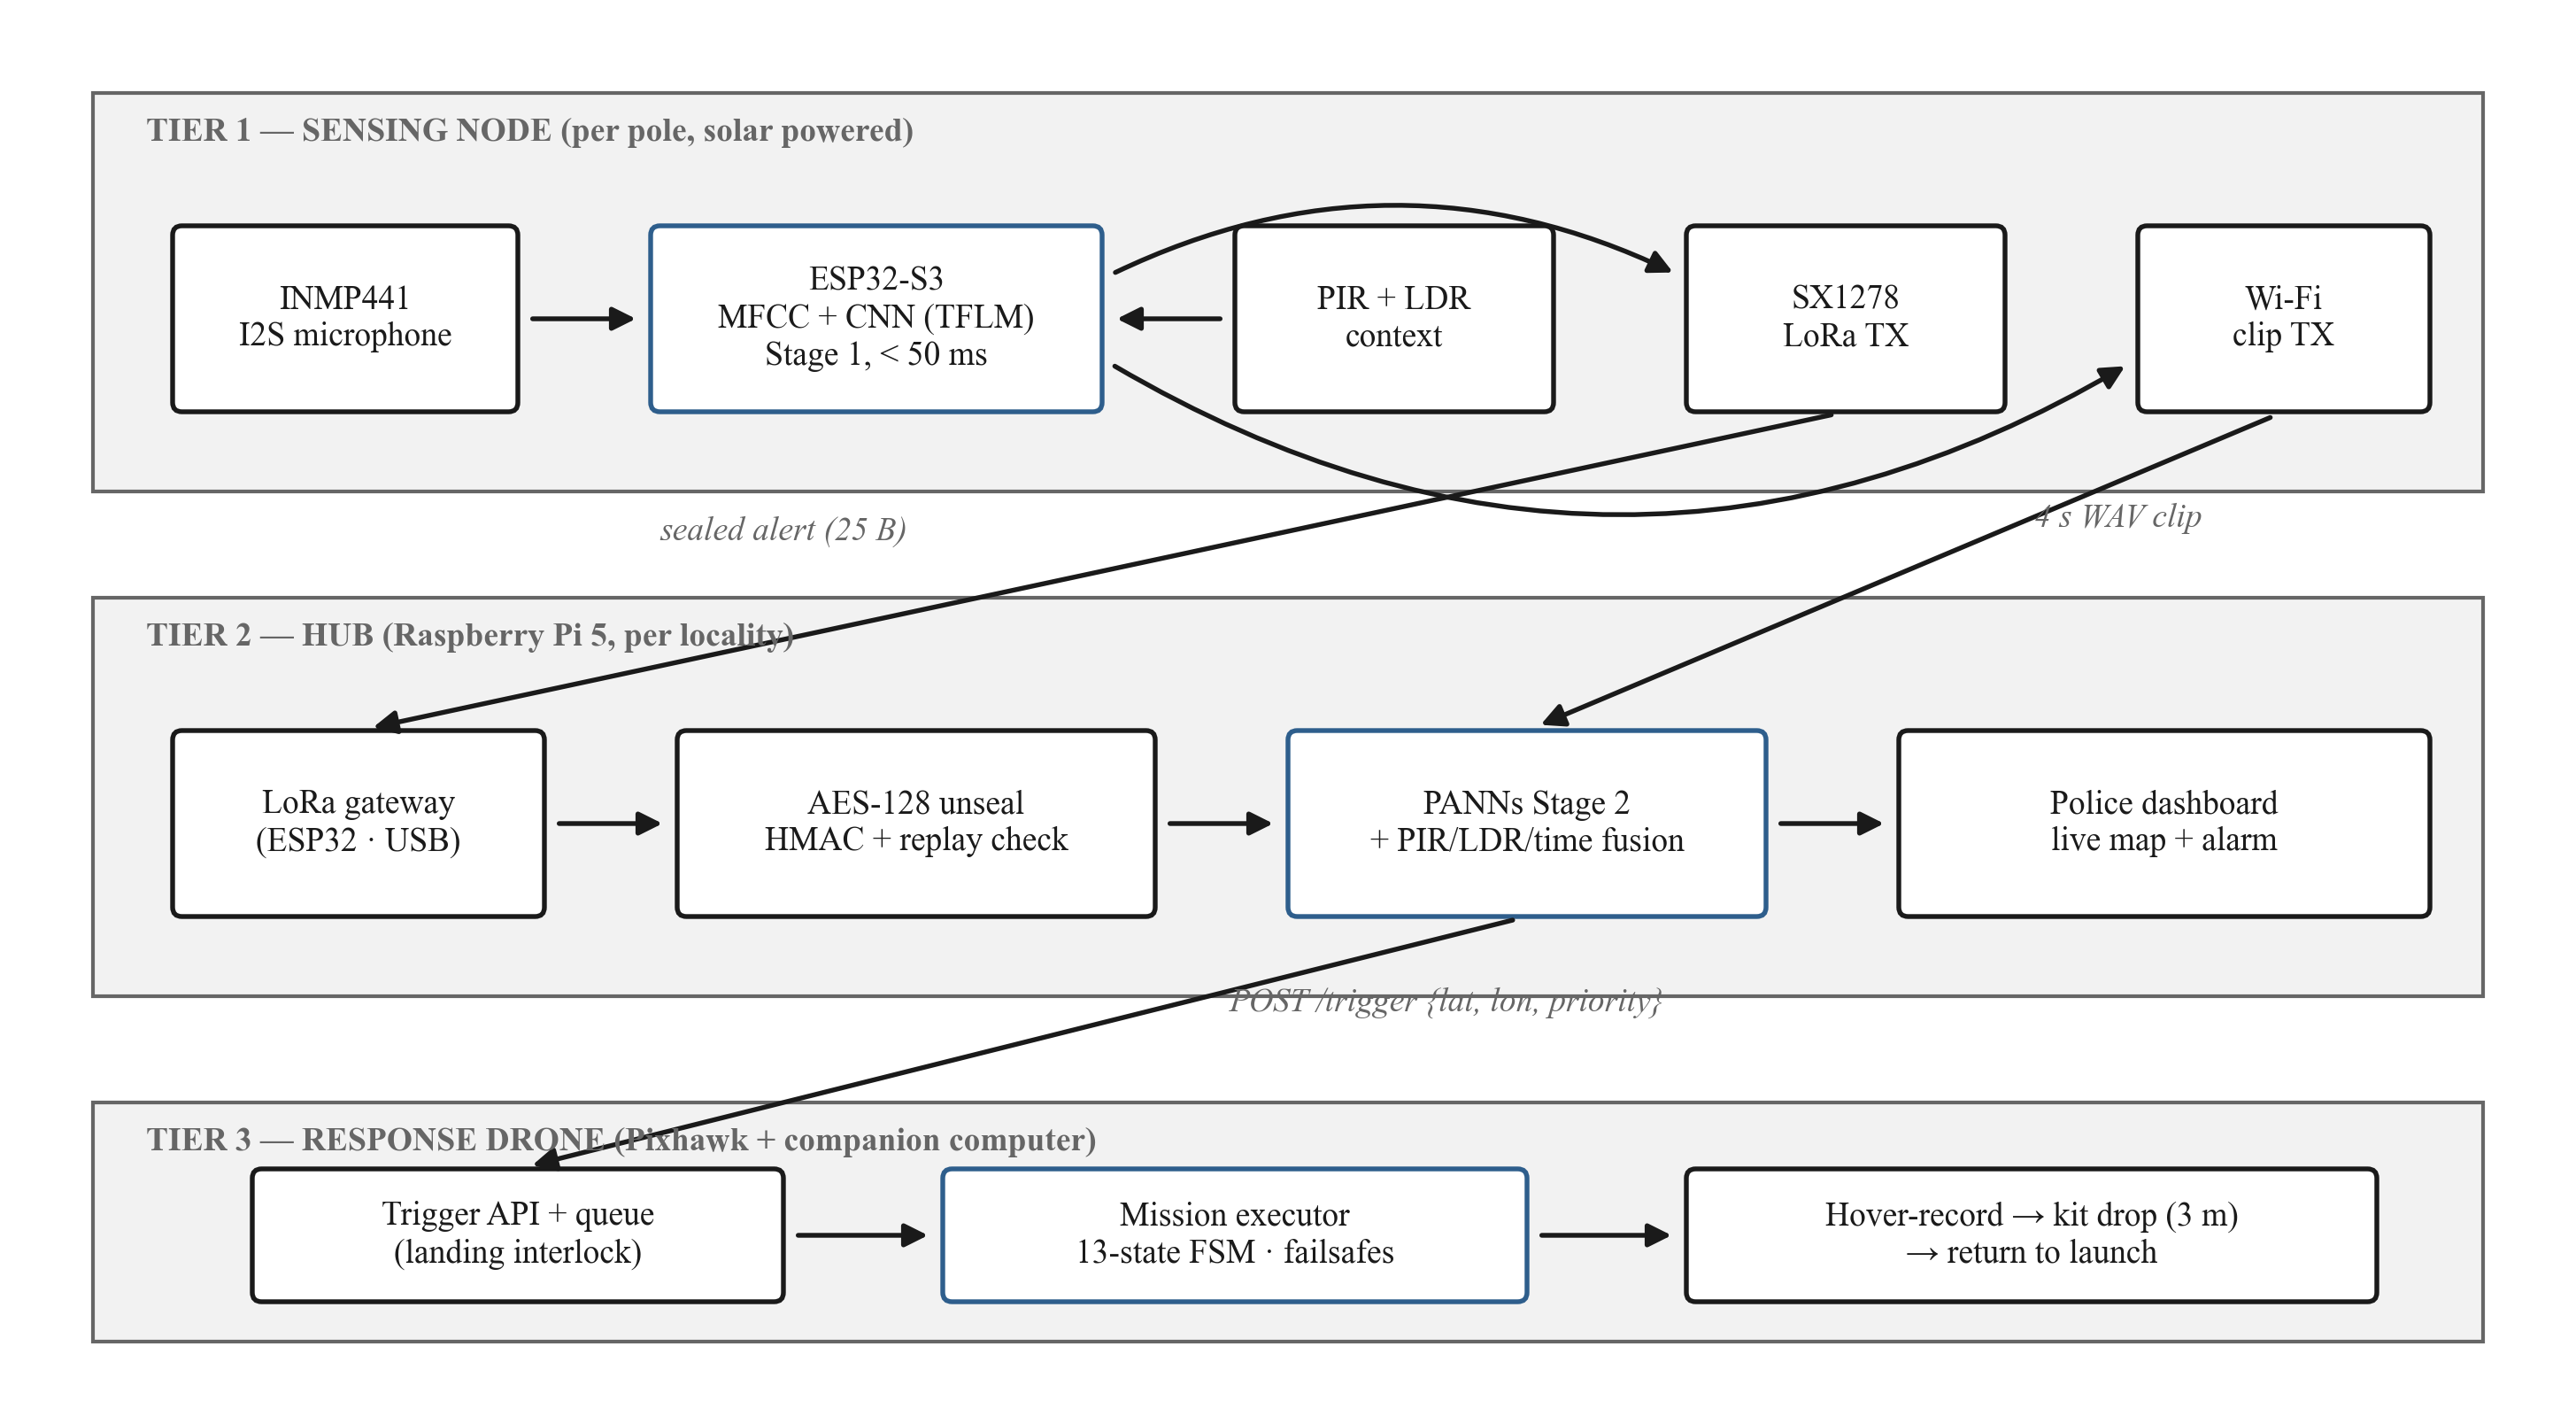
\includegraphics[width=\textwidth]{fig1_architecture.png}
\caption{VanniKawachh three-tier system architecture: per-pole solar
sensing nodes, the per-locality Raspberry Pi~5 hub, and the autonomous
response drone.}
\label{fig:architecture}
\end{figure}

\begin{small}
\begin{verbatim}
+------------- SENSING NODE (per pole, solar) --------------+
| INMP441 I2S mic -> ESP32-S3: MFCC + tiny CNN (TFLM,<50ms) |
| PIR (HC-SR501) + LDR context ; Stage-1 hit -> alert+clip  |
+--------------+----------------------------+---------------+
     LoRa SX1278 (alert, AES-128)   ESP-NOW / WiFi (4 s clip)
               v                            v
+------------- HUB (Raspberry Pi 5, per locality) ----------+
| LoRa gateway (ESP32 + SX1278 on USB serial)               |
| Stage 2: PANNs (CNN14/CNN10) + PIR/LDR/time fusion score  |
| Node registry: node_id -> surveyed (lat, lon)             |
| Police dashboard (live map + alarm) ; alert log           |
+--------------+---------------------------------------------+
        POST /trigger {lat, lon, incident_type, priority}
               v
+------------- RESPONSE DRONE (v1 stack, unchanged core) ---+
| trigger_api (FastAPI queue) -> mission_executor (13-state |
| FSM, verified mode setter, failsafe arbiter, landing      |
| interlock, obstacle keep-out routing)                     |
| v2: HOVERING + camera record -> DELIVERING (SG90 kit drop |
|     from 3 m; fail -> RTL) -> RTL                         |
+------------------------------------------------------------+
\end{verbatim}
\end{small}

\noindent\emph{The VanniKawachh chain in schematic form
(cf.\ Figure~\ref{fig:architecture}). Each tier verifies before it
acts: the node screens, the hub confirms, the flight stack confirms
its own commands.}

\textbf{Tier 1 --- sensing node.} One per pole. An ESP32-S3
continuously frames 16~kHz mono audio from an INMP441 I2S microphone,
extracts MFCC features, and runs a tiny quantized CNN (TensorFlow Lite
Micro, \texttt{micro\_speech}-class) against the distress vocabulary:
scream, cry, and the ``help'' / ``bachao'' keyword family. Budget:
under 50~ms per frame. An HC-SR501 PIR sensor and an LDR provide
motion and ambient-light context sampled alongside. A Stage-1 hit
produces exactly two transmissions --- a sealed 25-byte alert over
LoRa, and a 4~s audio clip over ESP-NOW/WiFi --- and nothing
otherwise.

\textbf{Tier 2 --- hub.} One Raspberry Pi~5 per locality. A gateway
ESP32 with an SX1278 bridges LoRa to USB serial. The hub authenticates
and decrypts each packet, resolves the node's surveyed coordinates
from a registry, waits briefly for the WiFi clip, re-scores the audio
with PANNs, fuses the score with PIR/LDR/time evidence into a
severity, and --- only above two explicit thresholds --- dispatches
the drone and raises the police dashboard alarm. Every incident,
dispatched or not, is logged.

\textbf{Tier 3 --- response drone.} The group's v1 flight stack: a
FastAPI~\cite{fastapi} trigger surface, a priority mission queue, and
a mission-executor state machine supervised by a failsafe arbiter. v2
adds a camera recording window during hover and a DELIVERING phase
that descends to 3~m and releases a first-aid kit by servo. The
stack's safety core is untouched.

\section{Design decisions and rationale}
\label{sec:rationale}

\textbf{Fixed nodes carry no live GPS.} Each pole is surveyed once at
installation (NEO-6M or a phone fix); the hub's registry maps
\texttt{node\_id} $\rightarrow$ (lat, lon, name). The LoRa packet
therefore carries two bytes of identity instead of a coordinate pair
--- smaller, and unspoofable at the position level: a node has no GPS
to jam, drift, or forge. An unknown \texttt{node\_id} is dropped at
the hub.

\textbf{LoRa carries the alert; WiFi carries the audio.} LoRa's
${\sim}$1--5.5~kbps cannot move a clip in useful time, so the
transports split: the sealed alert goes over LoRa instantly
(dead-zone-capable, kilometre-scale), and the 4~s verification clip
follows over ESP-NOW/WiFi (${\sim}$250~kbps, hundreds of metres
line-of-sight).

The split is a direct consequence of LoRa's physical layer. The
duration of one LoRa symbol at spreading factor SF over bandwidth BW
is
\begin{equation}
\label{eq:symtime}
T_s = \frac{2^{\mathrm{SF}}}{\mathrm{BW}}
\end{equation}
so higher spreading factors buy sensitivity --- the receiver's minimum
detectable signal being
\begin{equation}
\label{eq:sens}
P_{\min}\ [\mathrm{dBm}] = -174 + 10\log_{10}(\mathrm{BW}) +
\mathrm{NF} + \mathrm{SNR}_{\min}
\end{equation}
where NF is the receiver noise figure and $\mathrm{SNR}_{\min}$ the
demodulation threshold for the chosen SF --- at the price of airtime.
Evaluating the standard LoRa time-on-air formula for the system's
25-byte packet at SF9, 125~kHz bandwidth, coding rate 4:5 gives
approximately \textbf{0.21~s} of airtime per alert; moving a 4~s,
16~kHz, 16-bit clip (128~kB) over the same link would take on the
order of \emph{minutes}. Hence alert-on-LoRa, clip-on-WiFi: the
safety-critical 25 bytes ride the long-range dead-zone-capable
channel, and the bulk audio rides the short-range fast one.

The design degrades gracefully: if the clip never arrives within the
configured wait (8~s), the hub falls back to the Stage-1 confidence at
a haircut ($\times\,0.6$) --- enough to log always, and to dispatch
only if the evidence is otherwise strong. Multi-node corroboration
slots into the same fallback point as future work.

\textbf{Stage 1 is recall-tuned; Stage 2 is precision-tuned.} The
node's job is to \emph{never miss} a real event; its false positives
are expected and cheap, because the hub filters them with a model
three orders of magnitude larger, plus environmental evidence. This
division mirrors the economics: waking the hub costs milliwatts;
launching the drone costs a mission. The philosophy is the v1 flight
stack's \emph{verified dispatch} applied to sound.

\textbf{Every LoRa packet is sealed.} A spoofed packet would launch a
drone. \S\ref{sec:packetsecurity} details the AES-128-CTR + HMAC +
replay-counter construction.

\textbf{The flight core is untouched.} All v1 safety machinery ---
verified mode setter, failsafe arbiter, landing interlock, geofence,
stall detection, obstacle keep-out routing --- carries over unchanged.
It is the reason the response half of this project already works, and
Chapter~\ref{ch:response} documents it as the response layer.

\section{The mission lifecycle (response tier)}
\label{sec:lifecycle}

The executor's state machine threads IDLE $\rightarrow$ CONNECTING
$\rightarrow$ WAITING\_GPS $\rightarrow$ ARMING $\rightarrow$ TAKEOFF
$\rightarrow$ ENROUTE $\rightarrow$ HOVERING $\rightarrow$
\textbf{DELIVERING} $\rightarrow$ RTL $\rightarrow$ LANDED
$\rightarrow$ COMPLETED, with ABORTED and FAILED as abnormal terminals
--- thirteen states in v2 (DELIVERING is the addition). Three v1
properties are preserved: no state waits for human input; every
transition is timestamped into the mission log; every blocking loop
polls both the failsafe arbiter and the operator-cancel flag, so
abnormal termination is reachable from anywhere. The hover window
doubles as the evidence-recording window; DELIVERING runs only when
the mission requests a kit drop.

\section{Data flow, end to end}
\label{sec:dataflow}

Figure~\ref{fig:methodology} traces one incident through the system,
from the shout to the drone's return; the numbered steps below give
the corresponding software interfaces.

\begin{figure}[htbp]
\centering
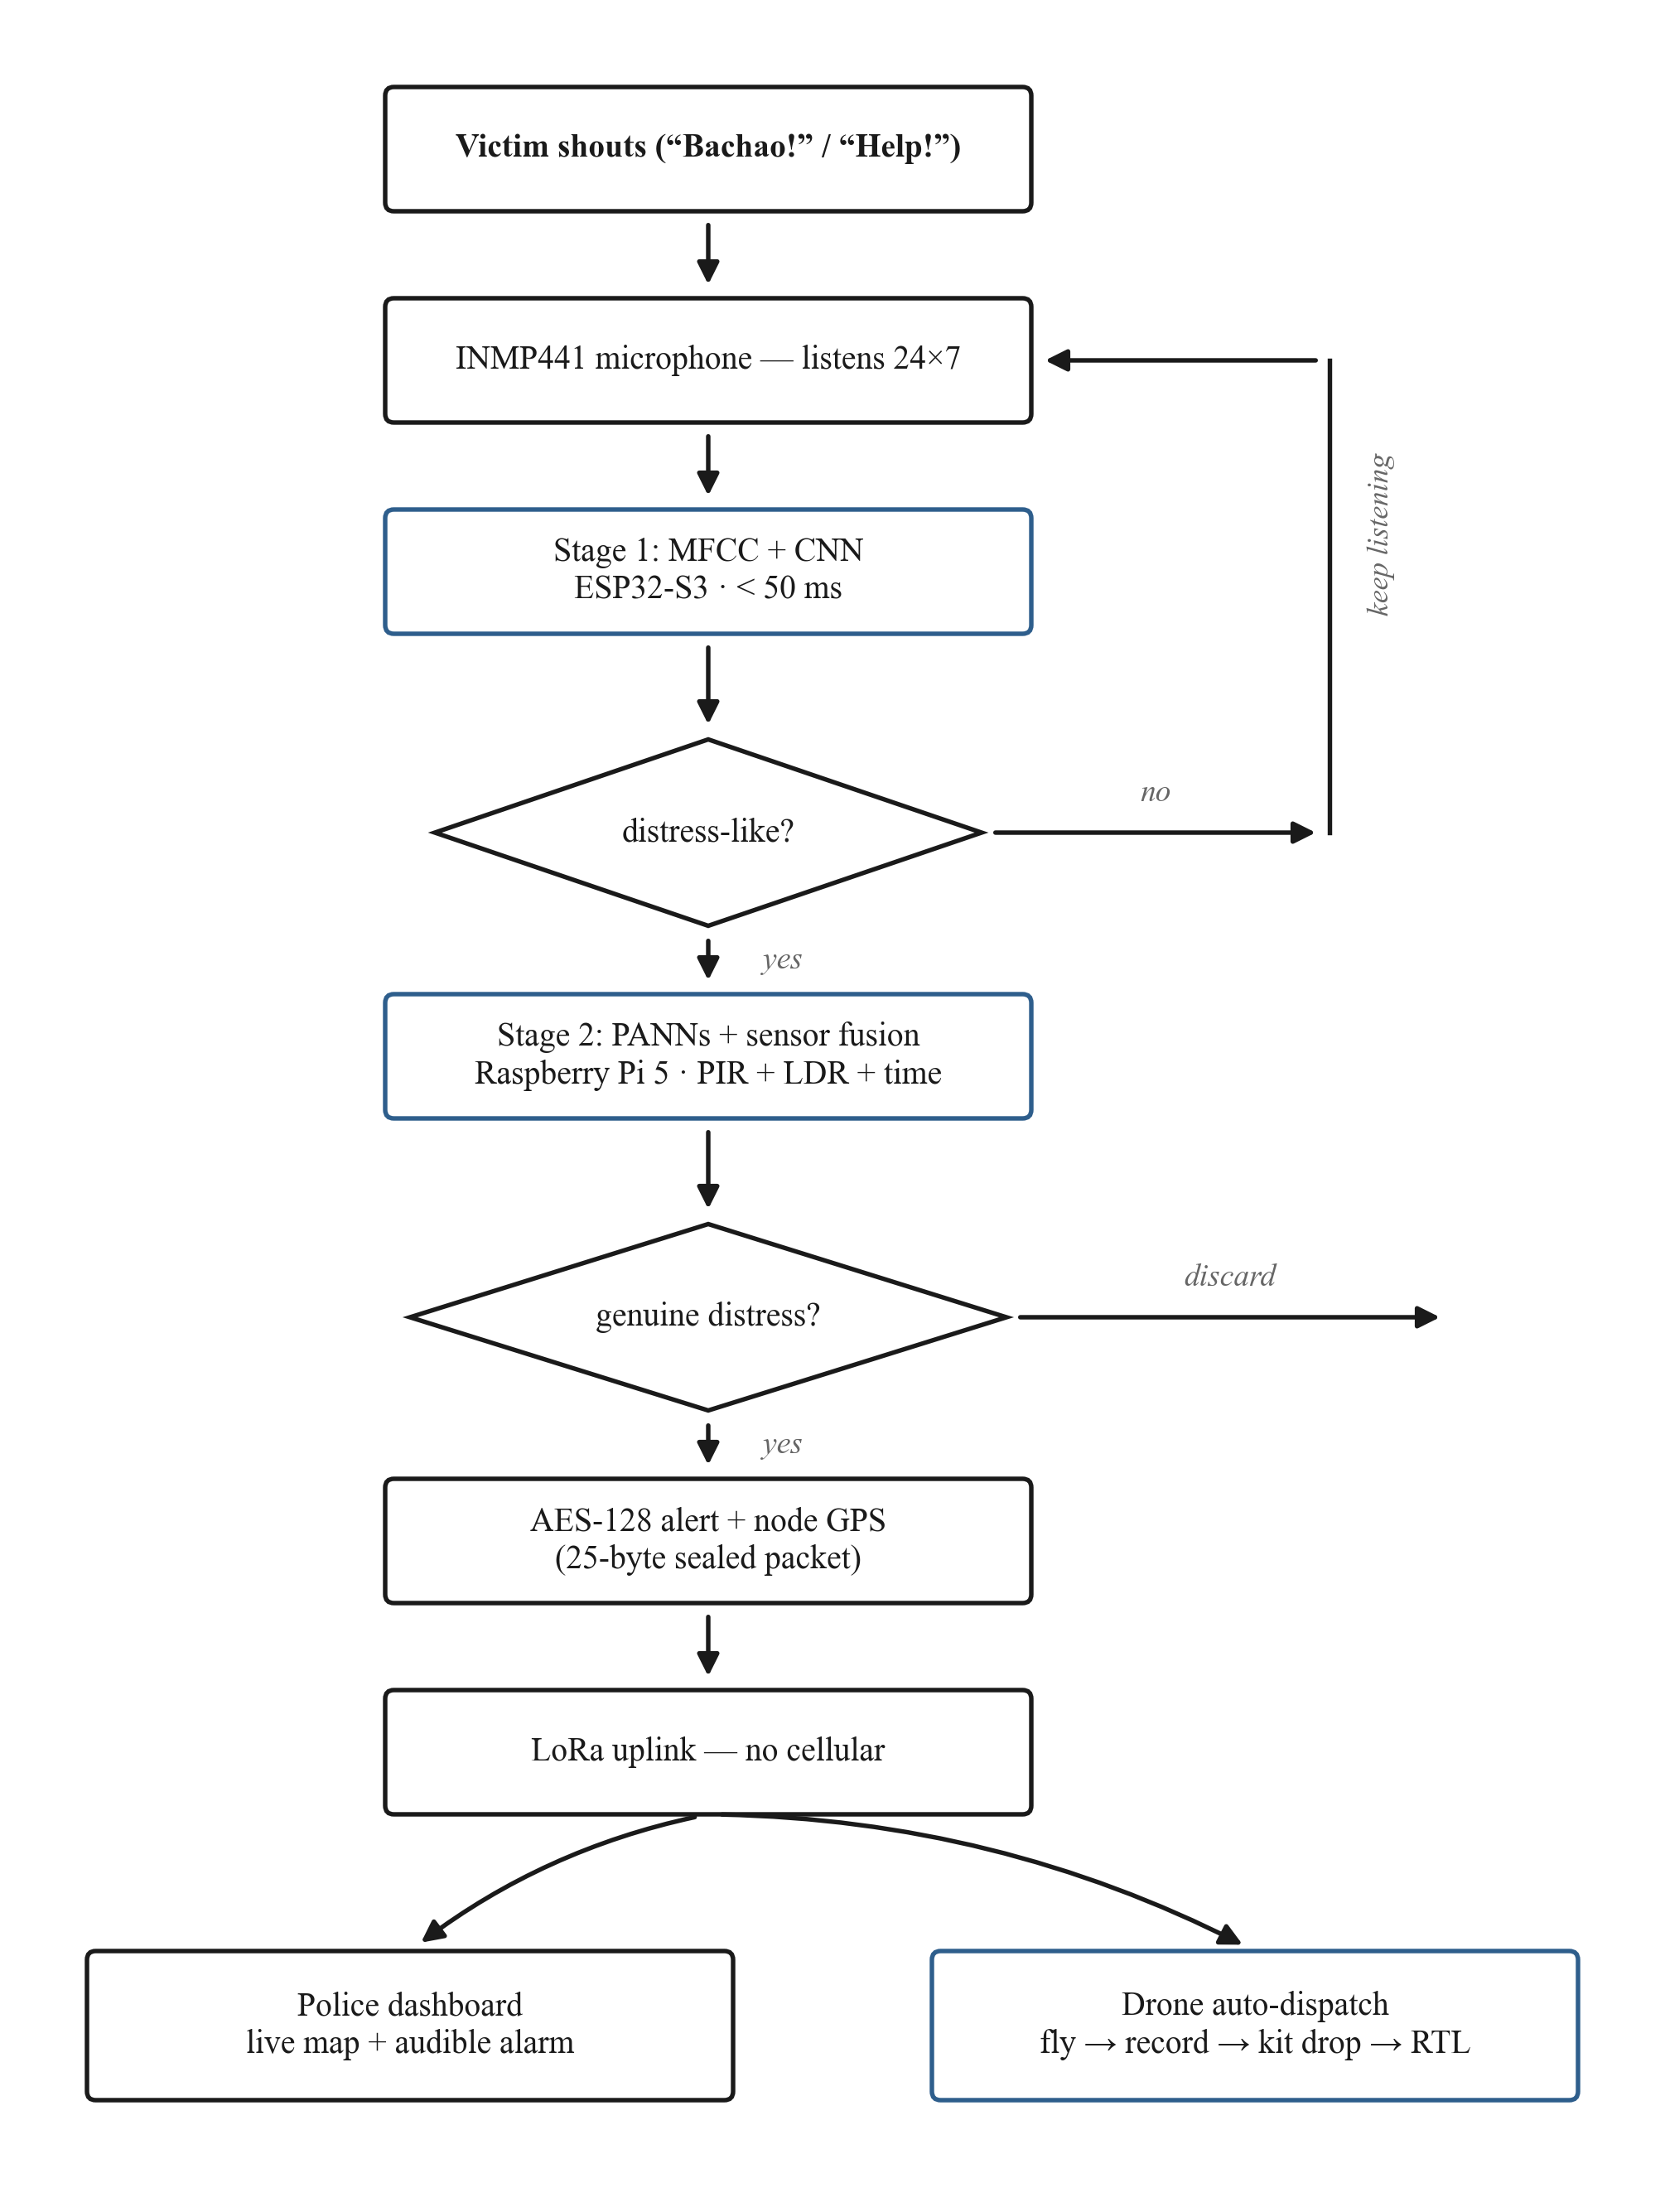
\includegraphics[width=\textwidth]{fig2_methodology.png}
\caption{Methodology flow: from the victim's shout through Stage-1
screening, Stage-2 verification and fusion, the sealed LoRa alert, to
the police dashboard and the drone auto-dispatch.}
\label{fig:methodology}
\end{figure}

\begin{enumerate}
\item Node: Stage-1 hit $\rightarrow$ sealed alert (LoRa) + 4~s clip
  (WiFi).
\item Gateway ESP32: LoRa RX $\rightarrow$ one line per packet over
  USB serial. The gateway does no crypto and no parsing beyond framing
  --- all intelligence stays on the Pi, where it can be updated
  without reflashing.
\item Hub pipeline: unseal (MAC, replay) $\rightarrow$ registry lookup
  $\rightarrow$ wait for clip $\rightarrow$ Stage-2 score
  $\rightarrow$ fusion $\rightarrow$ threshold gate $\rightarrow$
  dispatch + log.
\item Drone stack: \texttt{POST /trigger \{lat, lon, incident\_type,
  priority\}} $\rightarrow$ queue $\rightarrow$ mission with
  hover-record and kit drop $\rightarrow$ RTL.
\item Dashboard (React~\cite{react} + Leaflet~\cite{leaflet} over
  OpenStreetMap~\cite{osm} tiles): the incident appears on the
  police-facing map with severity, reasons, and mission id; the
  mission is trackable live.
\end{enumerate}

% ================================================================ Chapter 4
\chapter{Implementation: Sensing Node and Hub}
\label{ch:node-hub}

\section{Node firmware (\texttt{firmware/node/})}
\label{sec:nodefirmware}

The sensing node is a single Arduino sketch for the
ESP32-S3~\cite{esp32s3} structured as the pipeline of
\S\ref{sec:threetiers}: I2S capture from the INMP441~\cite{inmp441} at
16~kHz mono; framing and MFCC feature extraction; the TFLite-Micro
Stage-1 model hook; PIR and LDR sampling; AES-sealed LoRa alert
transmission (SX1278, LoRa library by Sandeep Mistry); and the
ESP-NOW/WiFi clip upload to the hub's clip server. The alert carries
the event class (1 = scream, 2 = help\_keyword, 3 = cry, 4 = crash),
the Stage-1 confidence quantized to a byte, the PIR flag, the raw LDR
level, the node battery percentage, and the monotonic packet counter.
Figure~\ref{fig:pipeline} shows the Stage-1 pipeline as implemented on
the node.

\begin{figure}[htbp]
\centering
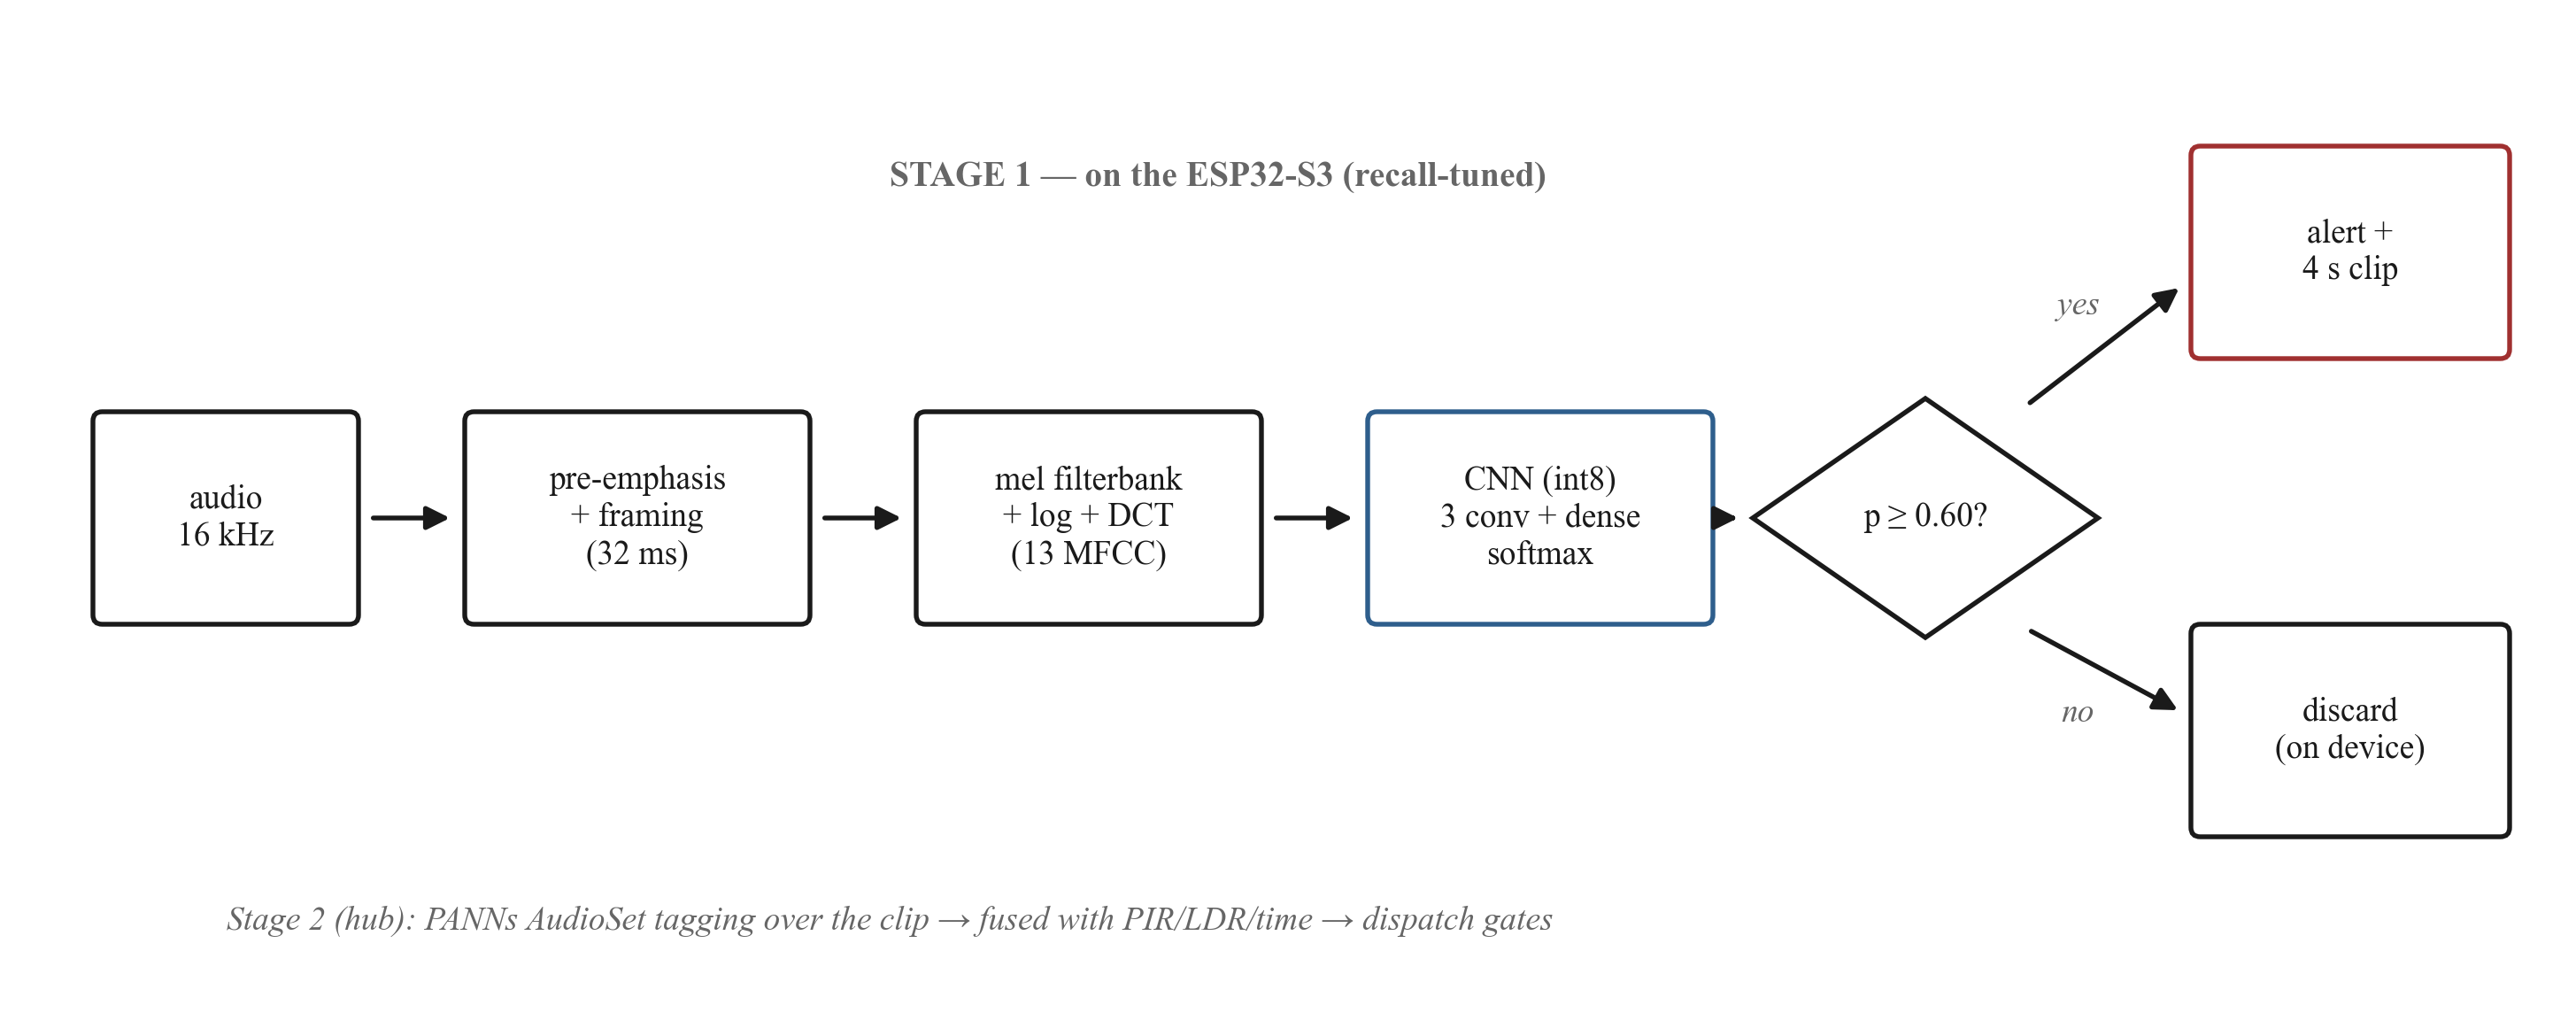
\includegraphics[width=\textwidth]{fig3_pipeline.png}
\caption{The two-stage acoustic pipeline. Stage~1 on the ESP32-S3
(recall-tuned): 16~kHz audio $\rightarrow$ pre-emphasis and 32~ms
framing $\rightarrow$ mel filterbank + log + DCT (13 MFCCs)
$\rightarrow$ int8 CNN $\rightarrow$ alert + clip on a hit, on-device
discard otherwise. Stage~2 on the hub runs PANNs tagging over the clip
and fuses it with PIR/LDR/time before the dispatch gates.}
\label{fig:pipeline}
\end{figure}

\textbf{The Stage-1 mathematics.} The feature front-end is the
classical MFCC chain. Each incoming frame is first pre-emphasized to
flatten the spectral tilt of speech,
\begin{equation}
\label{eq:preemph}
y[n] = x[n] - 0.97\,x[n-1]
\end{equation}
then windowed with a Hamming window of length $N$,
\begin{equation}
\label{eq:hamming}
w[n] = 0.54 - 0.46\cos\!\left(\frac{2\pi n}{N-1}\right)
\end{equation}
before the FFT. The power spectrum is pooled by a bank of $M$
triangular filters spaced uniformly on the mel scale,
\begin{equation}
\label{eq:mel}
m = 2595\,\log_{10}\!\left(1 + \frac{f}{700}\right)
\end{equation}
and the log energy of each filter output is taken,
\begin{equation}
\label{eq:fbank}
e_j = \log\!\left(\sum_{k} H_j(k)\,\lvert X(k)\rvert^2\right),
\qquad j = 1,\dots,M
\end{equation}
where $H_j$ is the $j$-th triangular filter. A DCT-II decorrelates the
log energies into the cepstral coefficients
\begin{equation}
\label{eq:dct}
c_i = \sum_{j=1}^{M} e_j
\cos\!\left[\,i\left(j - \tfrac{1}{2}\right)\frac{\pi}{M}\right],
\qquad i = 0,\dots,12
\end{equation}
of which the first \textbf{13} are retained as the frame's feature
vector.

The classifier head is a small CNN ending in a softmax over the $K$
event classes,
\begin{equation}
\label{eq:softmax}
p_k = \frac{e^{z_k}}{\sum_{j=1}^{K} e^{z_j}}
\end{equation}
trained (Phase~1) by minimizing the cross-entropy loss
\begin{equation}
\label{eq:xent}
\mathcal{L} = -\sum_{k=1}^{K} y_k \log p_k
\end{equation}
against one-hot labels $y$. For deployment under TensorFlow Lite Micro
the weights and activations are quantized to int8 with the affine map
\begin{equation}
\label{eq:quant}
x_q = \mathrm{round}\!\left(\frac{x}{s}\right) + z
\end{equation}
where $s$ is the per-tensor scale and $z$ the zero point --- the step
that shrinks the model into the ESP32-S3's RAM budget and the
$<$50~ms frame deadline.

\textbf{Status honesty.} The firmware's capture, sensing, sealing, and
transport paths are implemented; the Stage-1 \emph{model} is a hook.
Training the quantized MFCC + CNN on scream/cry/keyword data and
flashing it is Phase-1 work in progress (\S\ref{sec:notmeasured}).
Nothing in this thesis claims an on-device detection accuracy.

\section{Hub service (\texttt{hub/})}
\label{sec:hubservice}

The hub is a Python package on the Raspberry Pi~5~\cite{rpi5}, one
module per responsibility (Table~\ref{tab:hubmodules}).

\begin{table}[htbp]
\centering
\caption{Hub service modules and their responsibilities.}
\label{tab:hubmodules}
\small
\begin{tabular}{@{}lp{0.62\textwidth}@{}}
\toprule
\textbf{Module} & \textbf{Responsibility} \\
\midrule
\texttt{hub/config.py} & Env-driven settings: serial port, master
key, thresholds, drone API URL \\
\texttt{hub/node\_registry.py} & \texttt{node\_id} $\rightarrow$
(lat, lon, meta), JSON-backed; unknown id $\Rightarrow$ packet
dropped; tracks each node's last counter \\
\texttt{hub/packets.py} & 25-byte packet format; AES-128-CTR
seal/unseal, truncated HMAC-SHA256, replay counter
(\S\ref{sec:packetsecurity}) \\
\texttt{hub/lora\_gateway.py} & Reads the gateway ESP32's USB serial
stream; \texttt{--sim} mode substitutes synthetic packets \\
\texttt{hub/clip\_server.py} & Receives the nodes' 4~s WAV clips over
WiFi \\
\texttt{hub/verifier.py} & Stage-2 scoring: PANNs backend, or an
energy-heuristic dev fallback (\S\ref{sec:stage2}) \\
\texttt{hub/fusion.py} & Severity fusion of audio score with
PIR/LDR/time evidence (\S\ref{sec:fusion}) \\
\texttt{hub/pipeline.py} & The gate: alert $\rightarrow$ verify
$\rightarrow$ fuse $\rightarrow$ dispatch decision; no dispatch below
threshold \\
\texttt{hub/dispatcher.py} & POSTs \texttt{/trigger} to the drone
stack with the node's surveyed coordinates \\
\texttt{hub/main.py} & Entrypoint: \texttt{python -m hub.main}
(serial) or \texttt{--sim} \\
\bottomrule
\end{tabular}
\end{table}

The pipeline (\texttt{process\_packet}) executes the full chain for
one sealed packet: authenticate + decrypt + replay-check; registry
lookup (bump the node's counter only after acceptance); wait up to 8~s
for the clip at \texttt{hub/clips/<node\_id>\_<counter>.wav}; Stage-2
score the clip --- or, if the clip never arrives, substitute the
degraded audio score
\begin{equation}
\label{eq:degraded}
a = 0.6\,c
\end{equation}
where $c$ is the Stage-1 confidence (the no-clip haircut of
\S\ref{sec:rationale}); fuse; then gate: dispatch requires
\textbf{both} \texttt{audio\_score} $\geq 0.50$
(\texttt{VERIFY\_THRESHOLD}) \textbf{and} \texttt{severity}
$\geq 0.60$ (\texttt{DISPATCH\_THRESHOLD}). Below either threshold the
incident is logged with its reasons and no drone flies. Every incident
--- dispatched or not --- is appended to the incident list that feeds
the dashboard.

\section{Packet security (\texttt{hub/packets.py})}
\label{sec:packetsecurity}

The threat model is blunt: a spoofed packet launches a drone; an
eavesdropped packet reveals an incident in progress; a replayed packet
re-launches a drone at an attacker's chosen time. The wire format
(25 bytes, one comfortable LoRa frame; Figure~\ref{fig:packet}, full
layout in Appendix~\ref{app:packet}) answers all three:

\begin{figure}[htbp]
\centering
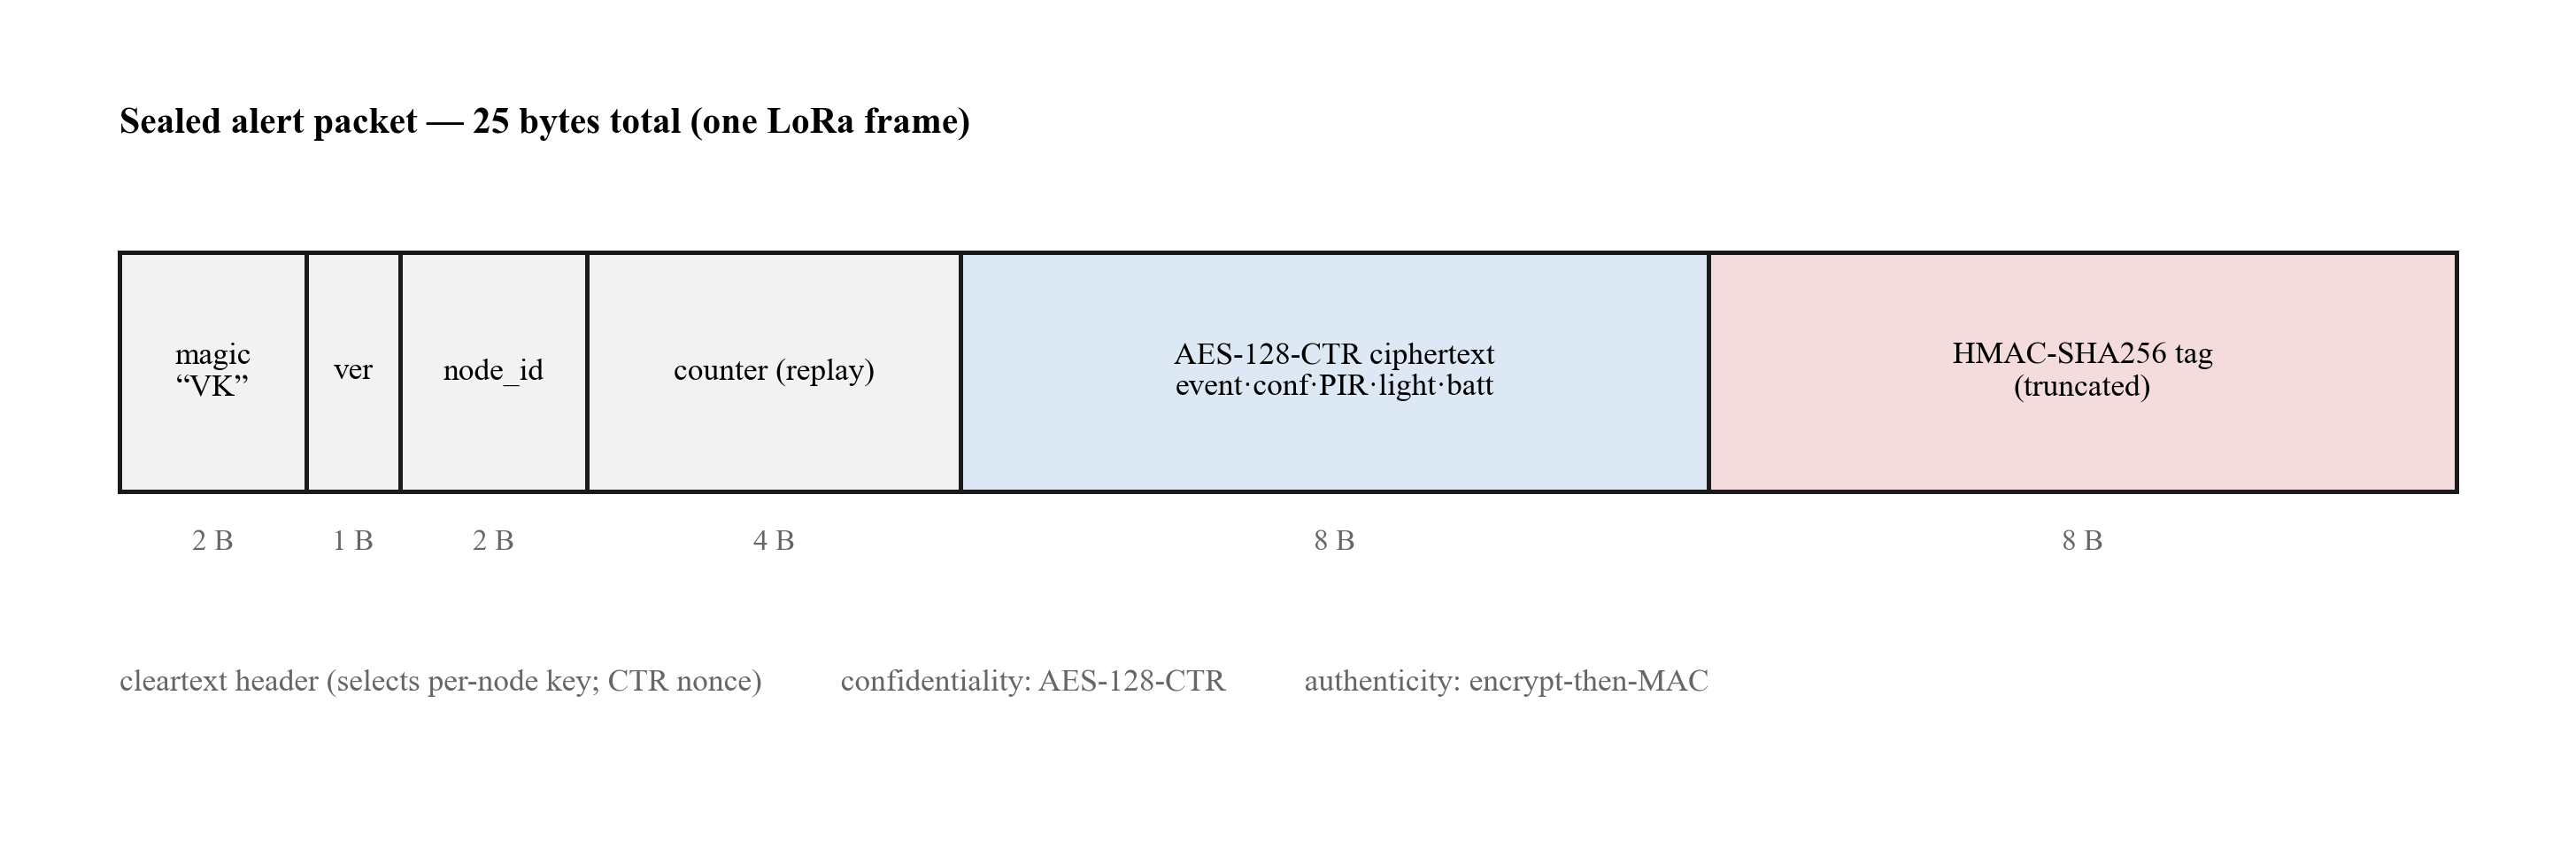
\includegraphics[width=0.9\textwidth]{fig4_packet.png}
\caption{The sealed 25-byte alert packet: cleartext header (magic,
version, node\_id, counter), AES-128-CTR ciphertext of the 8-byte
payload, and the truncated HMAC-SHA256 tag.}
\label{fig:packet}
\end{figure}

\begin{itemize}
\item \textbf{Confidentiality:} the 8-byte payload (event, confidence,
  PIR, light, battery) is AES-128-CTR encrypted. The CTR nonce is
  derived from the cleartext header (magic, version, node\_id,
  counter), unique per packet as long as the counter is monotonic.
\item \textbf{Authenticity:} an 8-byte MAC --- HMAC-SHA256 over header
  + ciphertext, truncated --- using the per-node key. A bad MAC is
  dropped before decryption is trusted.
\item \textbf{Replay protection:} the uint32 counter is monotonic per
  node; the hub rejects any counter $\leq$ the last accepted value for
  that node.
\item \textbf{Key management:} each node key is derived as
  \texttt{HMAC-SHA256(master\_key,} \texttt{"node:<id>")[:16]}, so
  provisioning a node requires only the
  master key and its id; the hub holds one secret.
\end{itemize}

\texttt{node\_id} and \texttt{counter} travel in cleartext by
necessity (the id selects the key; the counter builds the nonce) ---
neither is sensitive, and both are covered by the MAC.

Formally, the construction is as follows. Node $n$'s key is derived
from the hub's master key $K_m$ as
\begin{equation}
\label{eq:keyderive}
K_n = \mathrm{HMAC\mbox{-}SHA256}\!\left(K_m,\
\texttt{"node:}n\texttt{"}\right)[0{:}16]
\end{equation}
so the hub holds one secret and each node holds only its own derived
key (HMAC per RFC~2104~\cite{rfc2104}). The 8-byte payload $P$ is
encrypted in counter mode,
\begin{equation}
\label{eq:ctr}
C = P \oplus E_{K_n}(\mathrm{IV})
\end{equation}
where $E$ is AES-128~\cite{fips197} and the initial counter block IV
is built from the cleartext header (magic, version, node\_id, counter)
--- unique per packet as long as the node's counter is monotonic. The
authentication tag is an encrypt-then-MAC over everything on the wire,
\begin{equation}
\label{eq:mac}
\mathrm{tag} = \mathrm{HMAC\mbox{-}SHA256}\!\left(K_n,\
\mathrm{header} \parallel C\right)[0{:}8]
\end{equation}
and the hub accepts a packet if and only if
\begin{equation}
\label{eq:accept}
\mathrm{tag\ valid}\ \wedge\ \mathrm{counter} >
\mathrm{counter}_{\mathrm{last}}
\end{equation}
for that node, bumping $\mathrm{counter}_{\mathrm{last}}$ only after
acceptance. The truncated 8-byte tag leaves a blind-forgery success
probability of $2^{-64}$ per attempt --- negligible at LoRa alert
rates, a trade-off revisited if the channel is ever widened.

\section{Stage-2 verification (\texttt{hub/verifier.py})}
\label{sec:stage2}

Two interchangeable backends behind one interface
(\texttt{verify\_wav(path)} $\rightarrow$ score in $[0, 1]$):

\begin{itemize}
\item \textbf{PANNs (production).} The pretrained AudioSet tagging
  model (\texttt{panns-inference}, CNN14 by default; CNN10 or a
  MobileNet variant if the Pi is slow). The distress score is the
  summed probability over the distress-relevant AudioSet classes
  (screaming, shouting, yelling, crying, wailing, groaning,
  whimpering), clamped to 1.0. No bespoke training is required --- the
  verifier leans on AudioSet scale, which is exactly what a
  per-locality hub can afford to run and a pole cannot.
\item \textbf{Energy heuristic (dev/SITL fallback).} Loud +
  high-spectral-centroid + bursty audio scores high (weights
  0.45/0.35/0.20). This backend exists so the entire chain runs on any
  machine with no torch installation. It is \textbf{not} a claim of
  detection accuracy, and every result produced with it is labelled as
  fallback --- including the Phase-0 numbers of
  Chapter~\ref{ch:testing}.
\end{itemize}

The fallback scorer is worth stating exactly, because it gates the
Phase-0 rehearsal. Over the clip's samples $x[n]$, $n = 1,\dots,N$, it
computes the loudness as the root-mean-square level
\begin{equation}
\label{eq:rms}
\mathrm{RMS} = \sqrt{\frac{1}{N}\sum_{n=1}^{N} x[n]^2}
\end{equation}
and the spectral centroid --- the ``brightness'' of the clip, high for
screams ---
\begin{equation}
\label{eq:centroid}
C = \frac{\sum_{k} f_k\,\lvert X(k)\rvert}{\sum_{k}\lvert X(k)\rvert}
\end{equation}
where $X(k)$ is the magnitude spectrum at frequency $f_k$. Together
with a burstiness term ($\mathrm{burst} \in [0,1]$, from the
envelope's peak-to-mean structure) the score is
\begin{equation}
\label{eq:fallbackscore}
\mathrm{score} = 0.45\,\min\!\left(1, \frac{\mathrm{RMS}}{0.15}\right)
+ 0.35\,\mathrm{clip}\!\left(\frac{C - 400}{1600},\,0,\,1\right)
+ 0.20\,\mathrm{burst}
\end{equation}
i.e.\ full loudness credit at RMS $\geq 0.15$ full scale, and centroid
credit ramping linearly from 400~Hz to 2~kHz.

\section{Evidence fusion (\texttt{hub/fusion.py})}
\label{sec:fusion}

A night-time scream in a dark spot with motion nearby is a different
animal from a daytime shout on a busy road. With $a$ the Stage-2 audio
score, $c$ the Stage-1 confidence, $p \in \{0,1\}$ the PIR motion
flag, $L \in [0,255]$ the LDR light level, and $n \in \{0,1\}$ the
night indicator (1 between 20:00 and 06:00), the fused severity is the
weighted sum (Figure~\ref{fig:fusionfig})
\begin{equation}
\label{eq:fusioneq}
S = 0.60\,a + 0.15\,c + 0.10\,p + 0.08\,d + 0.07\,n,
\qquad d = 1 - \frac{L}{255}
\end{equation}
clamped to $[0,1]$. Audio dominates by design; the environmental terms
nudge. The dispatch gate of \S\ref{sec:hubservice} is then the
conjunction
\begin{equation}
\label{eq:gate}
\mathrm{dispatch} \iff a \ge 0.50\ \wedge\ S \ge 0.60
\end{equation}
and the mission priority is
\begin{equation}
\label{eq:priority}
\mathrm{priority} = \mathtt{high} \iff S \ge 0.75\ \vee\
\left(a \ge 0.6\ \wedge\ p = 1\right)
\end{equation}
otherwise \texttt{normal}.

\begin{figure}[htbp]
\centering
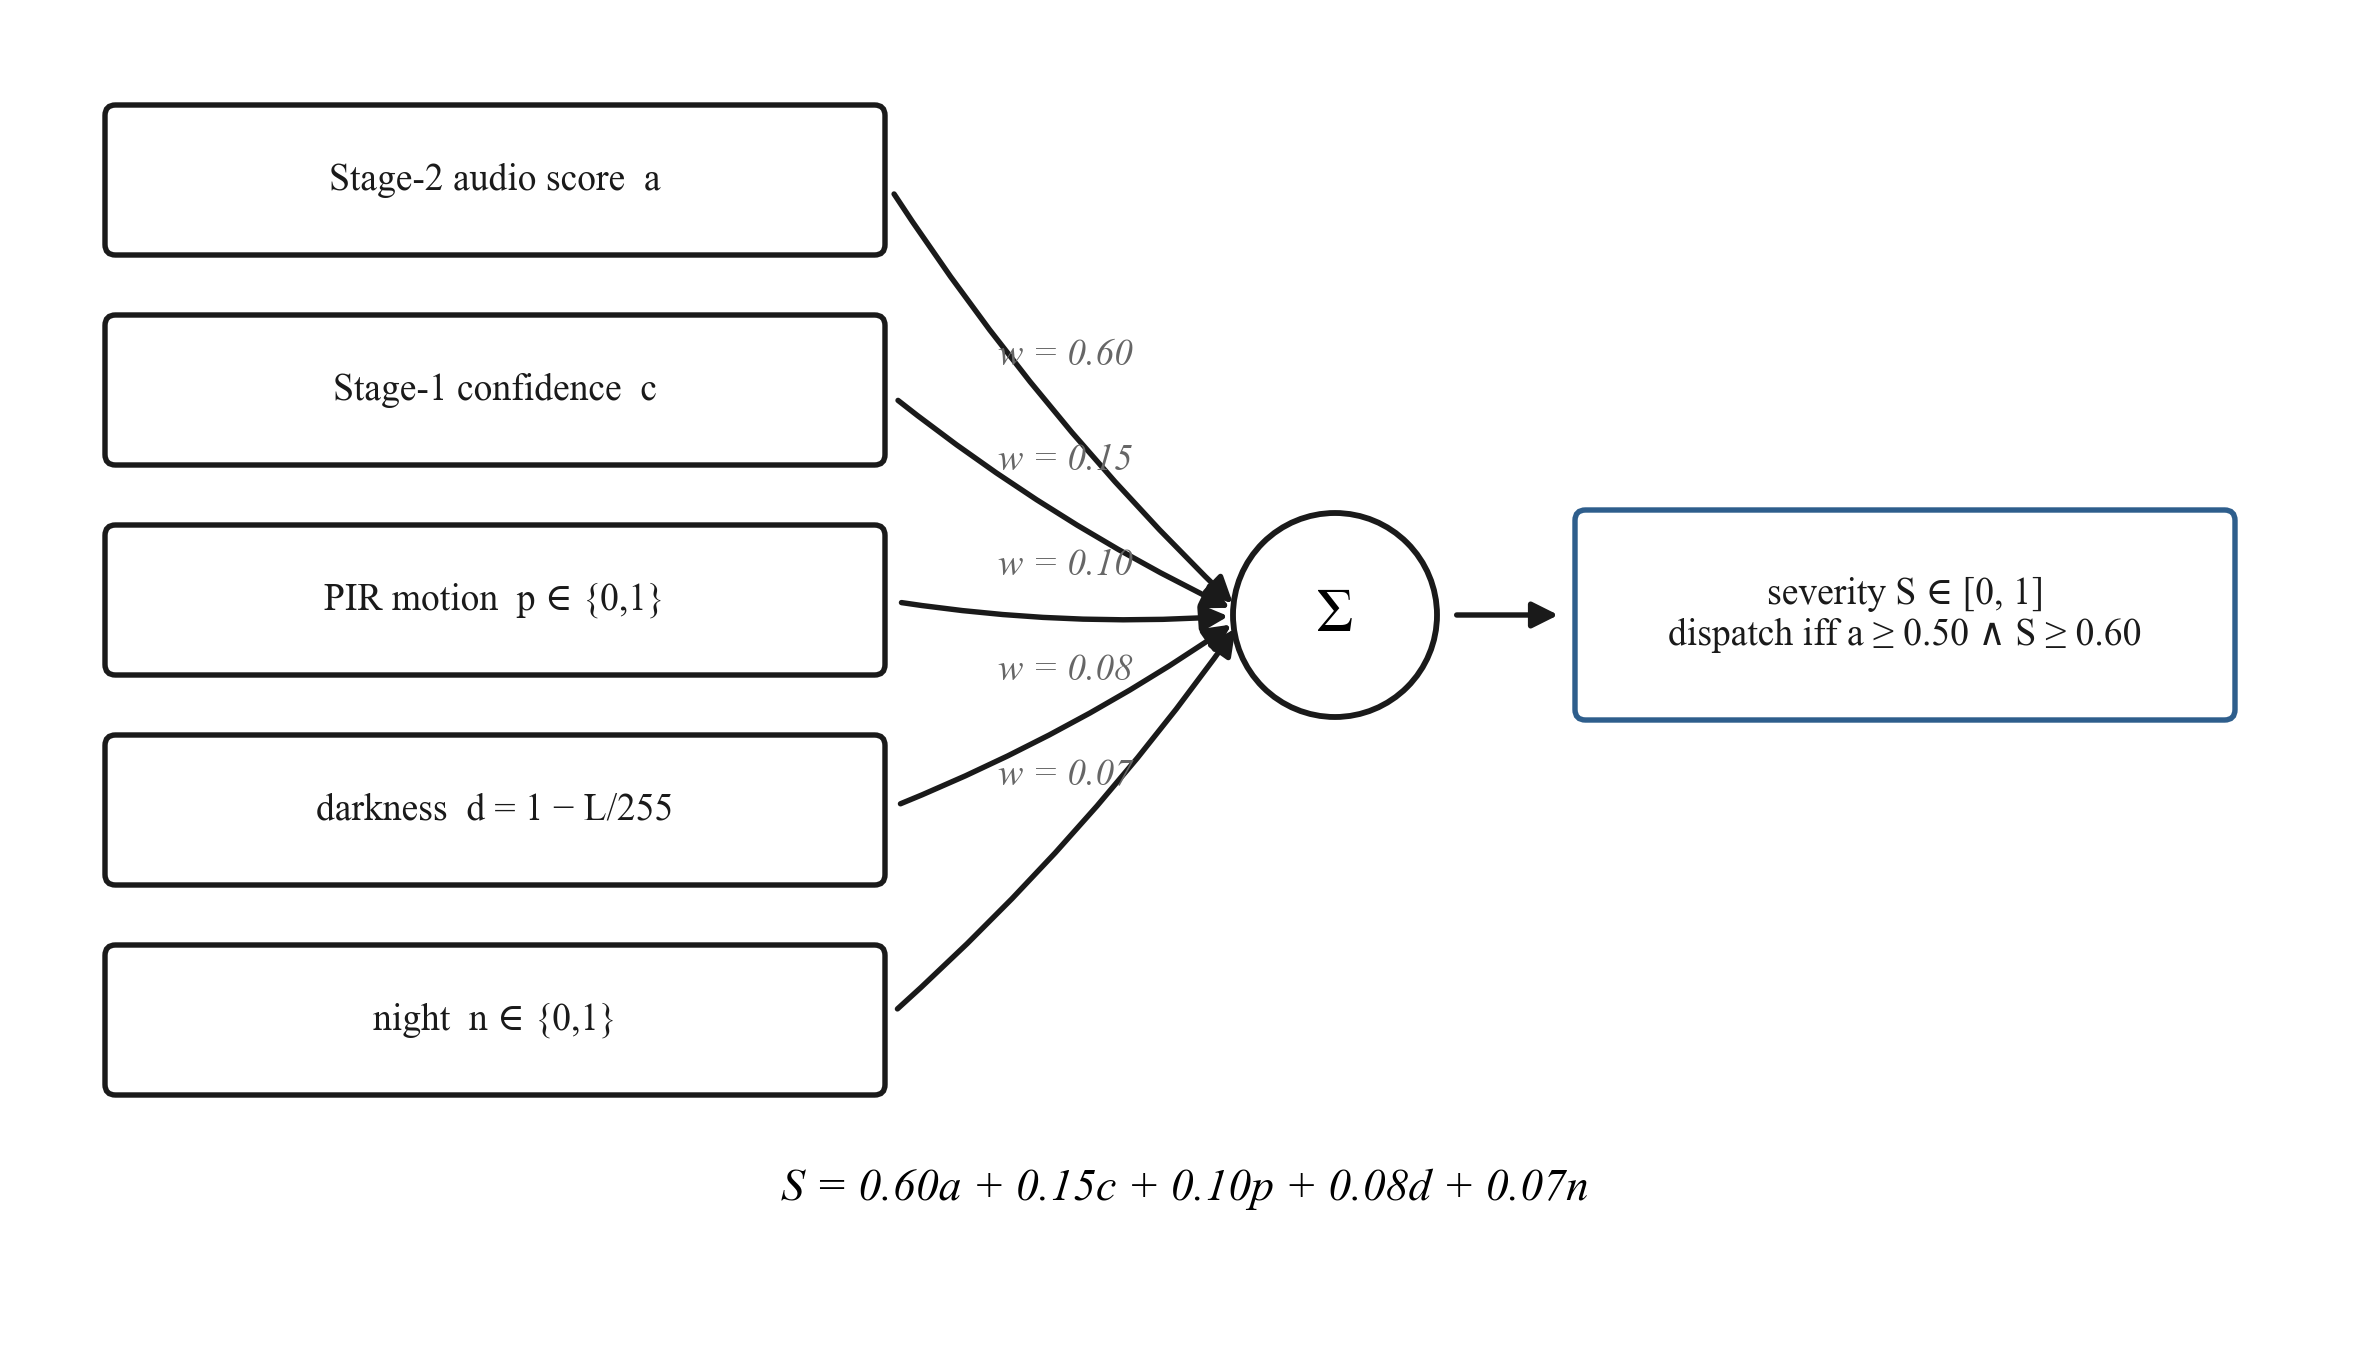
\includegraphics[width=\textwidth]{fig7_fusion.png}
\caption{Evidence fusion. The five evidence terms --- Stage-2 audio
score, Stage-1 confidence, PIR motion, darkness, and night --- are
combined with weights 0.60/0.15/0.10/0.08/0.07 into the severity $S$,
and dispatch requires both $a \ge 0.50$ and $S \ge 0.60$
(Eqs.~\ref{eq:fusioneq}--\ref{eq:gate}).}
\label{fig:fusionfig}
\end{figure}

Every fusion emits a human-readable reasons string
(\texttt{audio=\ldots\ stage1=\ldots\ pir=\ldots\ dark=\ldots\
night=\ldots}) that travels to the log and dashboard --- an operator
can always see \emph{why} a drone launched or an incident was held.
The weights are prototype values, stated as such, to be tuned against
Phase-1 bench data.

\section{Dispatch (\texttt{hub/dispatcher.py})}
\label{sec:dispatch}

On a gate-passing incident the dispatcher POSTs the v1 trigger API:
target = the node's surveyed coordinates, \texttt{incident\_type} from
the event class, \texttt{priority} from fusion, \texttt{deliver\_kit}
set. The drone stack's own edge validation (geofence, altitude bounds,
queue admission) applies unchanged --- the hub is a client of the same
hardened surface any operator would use, not a privileged backdoor.

% ================================================================ Chapter 5
\chapter[Implementation: The Response Layer (Safety-Verified
Autonomous Flight)]{Implementation: The Response Layer\\
(Safety-Verified Autonomous Flight)}
\label{ch:response}

The response layer is the group's v1 flight stack, built and validated
before the VanniKawachh pivot, and retained unchanged because its
properties are exactly what an unattended women-safety responder
needs. This chapter preserves the v1 technical record --- it is still
accurate --- and adds the two v2 extensions (camera, payload).
Figure~\ref{fig:fsm} shows the executor's thirteen-state mission state
machine (\S\ref{sec:lifecycle}), including the v2 DELIVERING phase.

\begin{figure}[htbp]
\centering
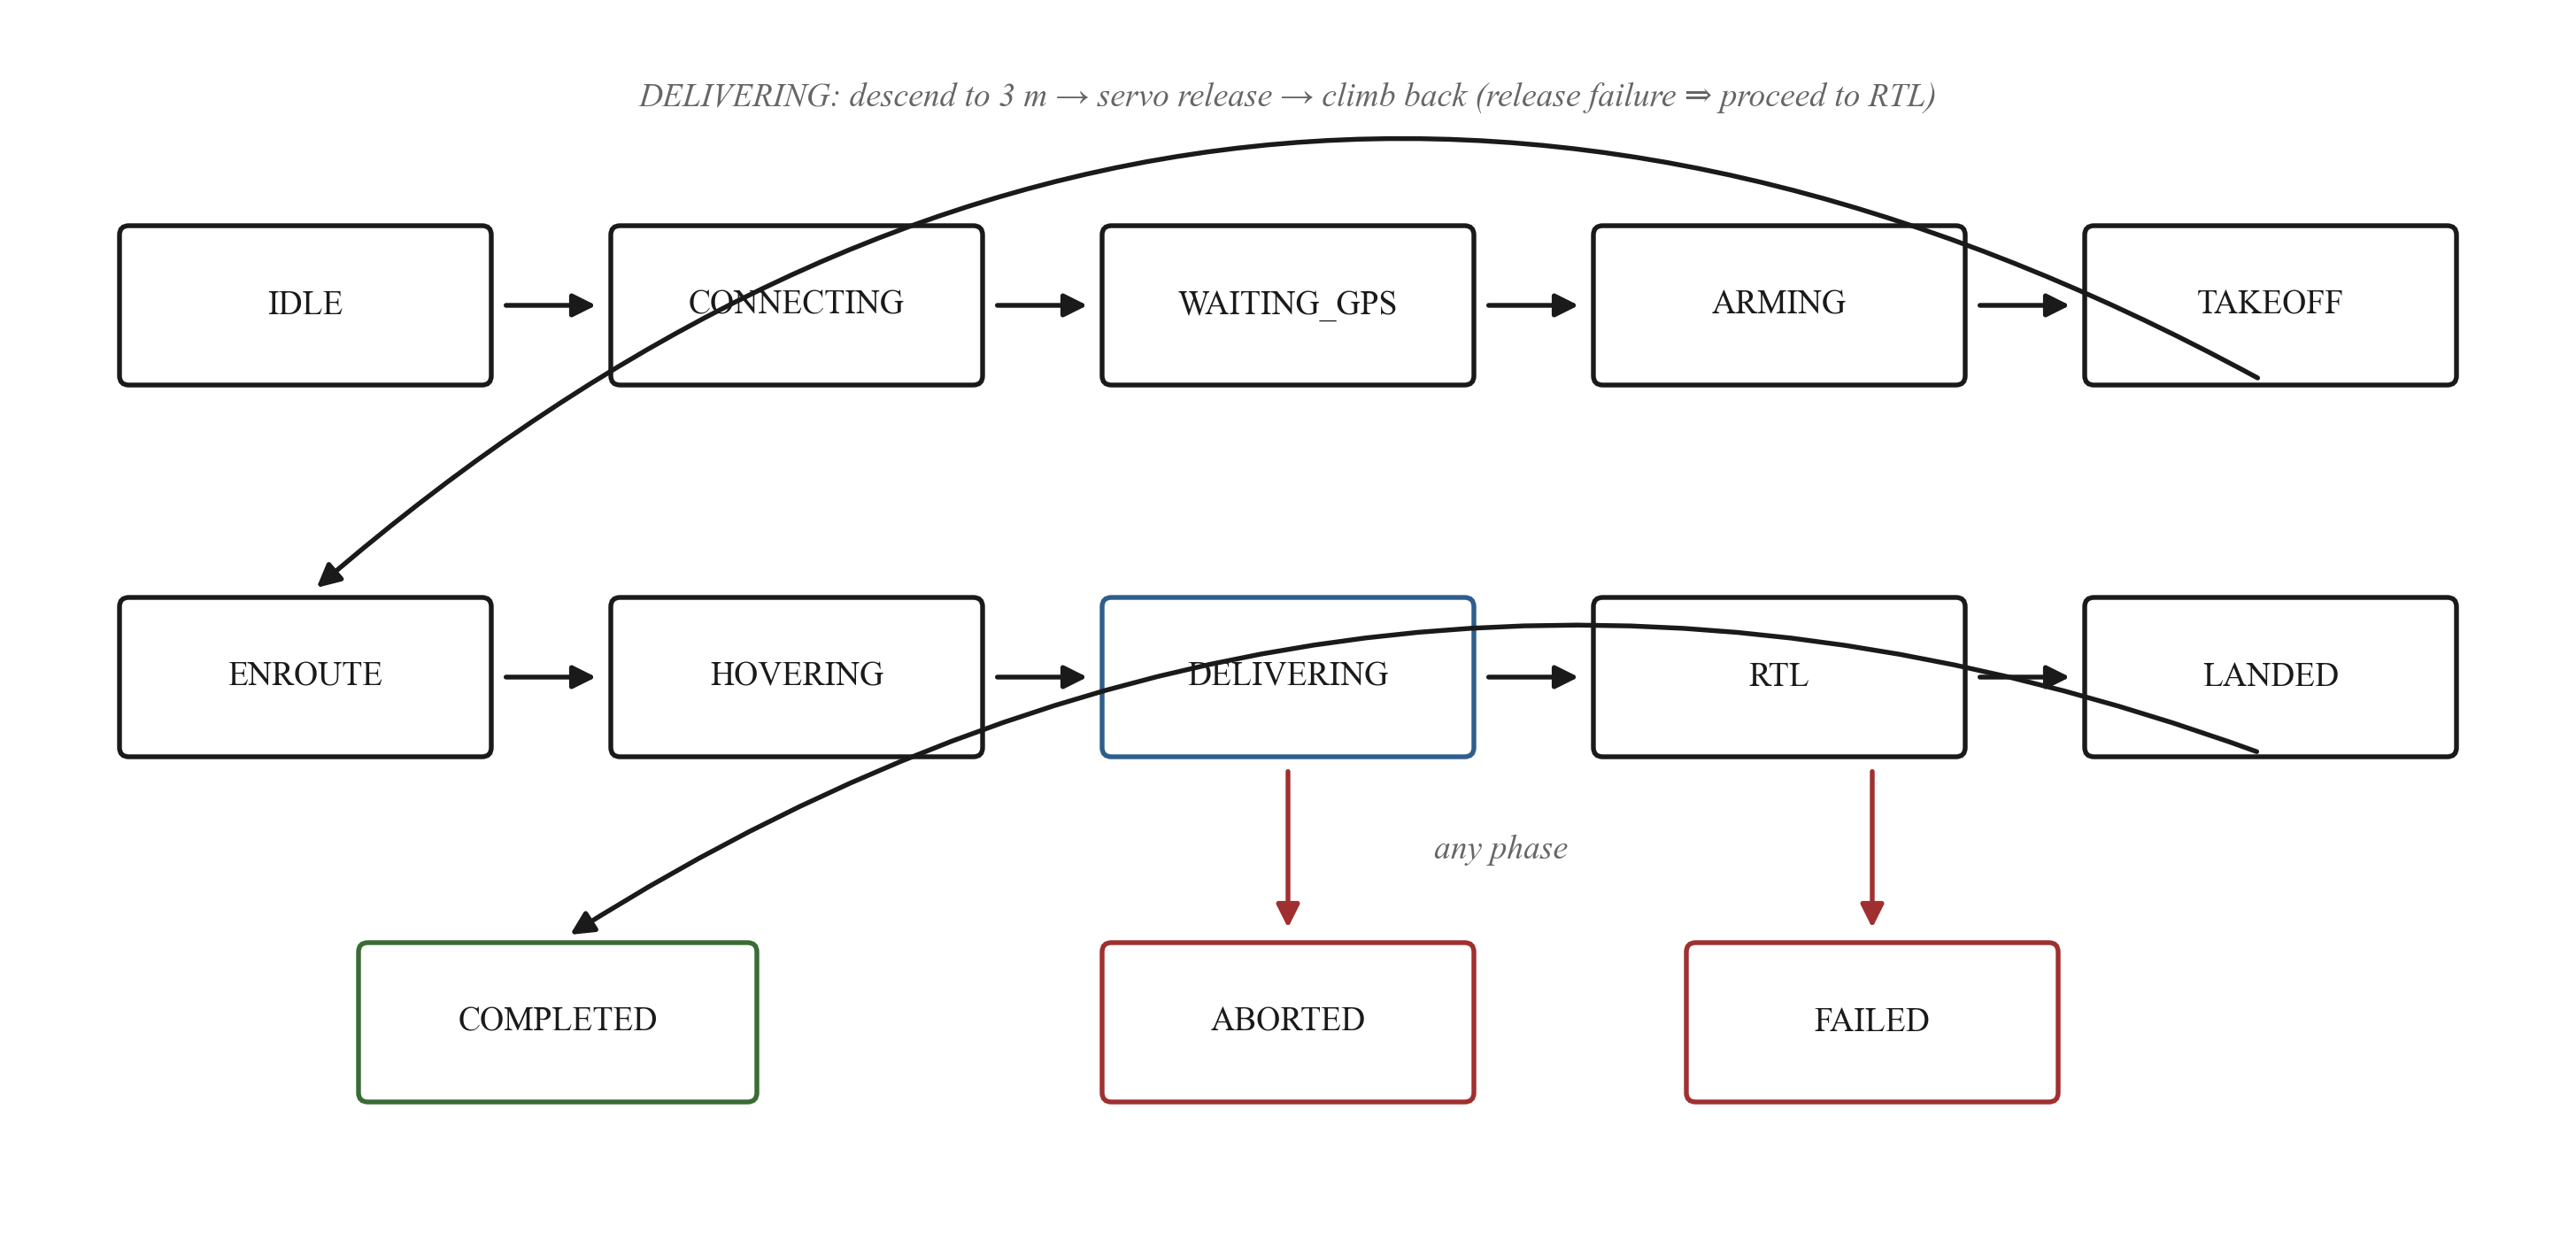
\includegraphics[width=\textwidth]{fig5_state_machine.png}
\caption{The mission executor's thirteen-state machine: IDLE
$\rightarrow$ CONNECTING $\rightarrow$ WAITING\_GPS $\rightarrow$
ARMING $\rightarrow$ TAKEOFF $\rightarrow$ ENROUTE $\rightarrow$
HOVERING $\rightarrow$ DELIVERING $\rightarrow$ RTL $\rightarrow$
LANDED $\rightarrow$ COMPLETED, with ABORTED and FAILED as abnormal
terminals reachable from every flight phase.}
\label{fig:fsm}
\end{figure}

\section{Hazard analysis}
\label{sec:hazards}

A compact HAZOP-style pass over the mission lifecycle yields the
hazard set the design must close (Table~\ref{tab:hazards}).

\begin{table}[htbp]
\centering
\caption{Hazard analysis of the mission lifecycle.}
\label{tab:hazards}
\small
\begin{tabular}{@{}lp{0.28\textwidth}p{0.28\textwidth}p{0.22\textwidth}@{}}
\toprule
\textbf{ID} & \textbf{Hazard} & \textbf{Worst credible outcome} &
\textbf{Closed by} \\
\midrule
H1 & Mode command silently rejected & Stranded/uncontrolled aircraft;
unrecallable mission & \S\ref{sec:verifiedmode} verified setter \\
H2 & Emergency command (RTL/LAND) not delivered & Failsafe ineffective
at the moment it matters & \S\ref{sec:verifiedmode} + cross-action
fallback \\
H3 & New mission starts while airborne & Takeoff commanded to flying
vehicle; undefined behaviour & \S\ref{sec:interlock} interlock \\
H4 & Transient GPS dropout treated as loss & Unnecessary landing on
unsafe ground & \S\ref{sec:arbiter} debounce \\
H5 & Critical battery during RTL & Aircraft presses home and falls
short & \S\ref{sec:arbiter} mid-return escalation \\
H6 & Demand downgraded (LAND$\rightarrow$RTL) & Wrong recovery flown &
\S\ref{sec:arbiter} monotone severity \\
H7 & Target beyond geofence accepted & Predictable mid-air abort;
wasted battery at distance & edge validation \\
H8 & Wind stall / rejected goto & Battery exhausted loitering &
leg-stall detector \\
H9 & Process shutdown mid-flight & Aircraft abandoned under autopilot
defaults & shutdown RTL \\
H10 & Dispatch by unauthorized party & Aircraft weaponized by anyone
on the network & token auth + sealed LoRa path
(Ch.~\ref{ch:node-hub}) \\
H11 & Kit-release failure at low altitude & Aircraft loiters at 3~m
over an incident scene & \S\ref{sec:delivering} fail $\rightarrow$
RTL rule \\
\bottomrule
\end{tabular}
\end{table}

\section{Verified mode transition}
\label{sec:verifiedmode}

Every flight-mode command, nominal or emergency, routes through one
routine, \texttt{\_set\_mode\_}\allowbreak\texttt{confirmed}: issue
through the high-level interface; loop until deadline reading the
autopilot's HEARTBEAT-derived mode; every 700~ms of non-confirmation
re-issue through
\texttt{COMMAND\_LONG(}\allowbreak\texttt{MAV\_CMD\_DO\_SET\_MODE)}
\emph{and} the legacy
\texttt{SET\_MODE} encoding and re-poke the high-level setter;
success iff the \emph{autopilot reports} the requested mode. Failure
on the abort path triggers the cross-action fallback: an unconfirmable
RTL becomes a LAND attempt and vice versa --- some confirmed recovery
beats an optimal unconfirmed one. Idempotence of mode-setting makes
the retry loop safe; reading confirmation from the autopilot's own
report makes it sound. The need is empirical: the standard client
idiom for entering GUIDED is silently ignored by the ArduCopter 3.3
simulator while reporting success (H1) --- observed in v1's first
flight, and the origin of the whole project's verification philosophy.
The bare setter appears nowhere outside the routine; a reviewer can
verify the property by grepping for mode assignments.

\section{The landing interlock}
\label{sec:interlock}

Two mechanisms, redundant by intent (Figure~\ref{fig:interlock}). The
\textbf{abort guarantee}: every abnormal termination (failsafe,
recall, exception with an airborne vehicle) commands its action
through \S\ref{sec:verifiedmode} and then blocks --- polling armed
state and relative altitude --- until disarm or a 240~s bound, before
the queue regains control. The \textbf{pre-flight check}: a dequeued
mission re-reads the armed flag and waits (bounded, 120~s) or fails
rather than arm an armed vehicle. Together they make the invariant ---
\emph{the queue can never start a flight against an airborne vehicle}
--- structural rather than probabilistic. The same property is
defended at process boundaries: shutdown with an armed vehicle
commands RTL (verified) before the MAVLink link drops (H9).

\begin{figure}[htbp]
\centering
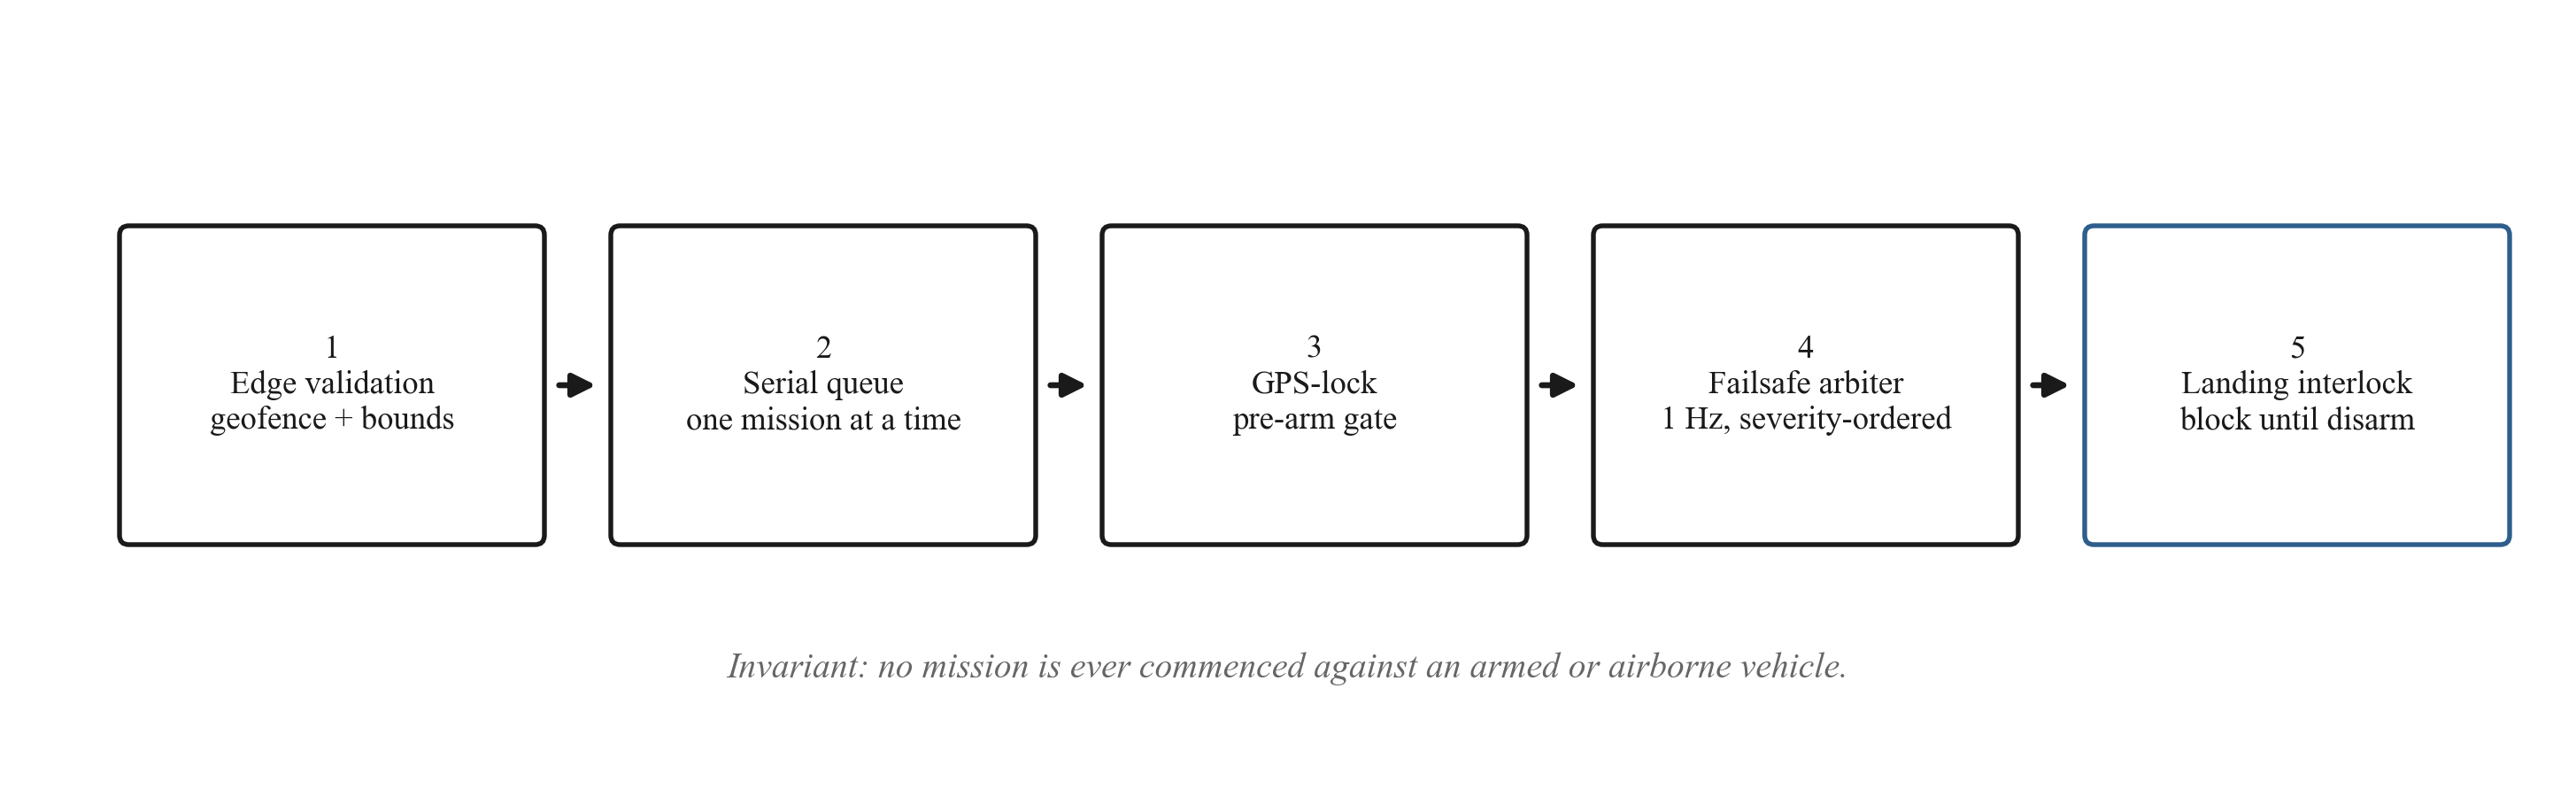
\includegraphics[width=\textwidth]{fig6_interlock.png}
\caption{The safety interlock chain: edge validation, queue admission,
the pre-flight armed check, failsafe arbitration in every blocking
loop, and the abort guarantee that blocks until disarm --- the gates a
dispatch must pass between network trigger and landing.}
\label{fig:interlock}
\end{figure}

\section{Failsafe arbitration}
\label{sec:arbiter}

The arbiter evaluates four condition families at 1~Hz --- battery low
(20\%) and critical (10\%), GPS fix validity, geofence distance,
mission wall-clock --- and maintains exactly one demanded action under
three rules. \textbf{Monotone severity:} demands only escalate (NONE
$<$ RTL $<$ LAND); H6 closed by construction. \textbf{Debounce:} GPS
loss fires only after $N$ (default 3) consecutive bad samples, reset
on recovery; it demands LAND because a return path is non-navigable
without positioning; H4 closed with detection latency bounded at $N$
seconds. \textbf{Fire-once:} each named hazard emits once per mission,
re-emission permitted only as escalation --- the incident record stays
a record. The executor couples to the arbiter inside every blocking
loop, \emph{including the RTL loop}, which re-reads the demand each
second and swaps to LAND on escalation (H5).

Two pieces of mathematics underpin the arbiter's inputs. The geofence
evaluator measures the vehicle's great-circle distance from home with
the haversine formula: for latitudes $\varphi_1, \varphi_2$ and
longitude difference $\Delta\lambda$,
\begin{equation}
\label{eq:haversine}
d = 2R \arcsin\sqrt{\sin^2\!\frac{\Delta\varphi}{2} +
\cos\varphi_1 \cos\varphi_2 \sin^2\!\frac{\Delta\lambda}{2}},
\qquad R = 6371\ \mathrm{km}
\end{equation}
--- the same computation used by edge validation (H7) and by the
acceptance harness's closest-approach metric. The GPS-fix validity the
arbiter debounces is itself the output of the autopilot's extended
Kalman filter, which maintains the state estimate $\hat{x}$ through
the standard predict/update pair
\begin{equation}
\label{eq:ekfpredict}
\hat{x}_{k|k-1} = F_k\,\hat{x}_{k-1|k-1}, \qquad
P_{k|k-1} = F_k P_{k-1|k-1} F_k^{\top} + Q_k
\end{equation}
\begin{equation}
\label{eq:ekfupdate}
\hat{x}_{k|k} = \hat{x}_{k|k-1} +
K_k\left(z_k - H_k\,\hat{x}_{k|k-1}\right),
\qquad
K_k = P_{k|k-1} H_k^{\top}\left(H_k P_{k|k-1} H_k^{\top} +
R_k\right)^{-1}
\end{equation}
fusing GPS, IMU, and barometer. The companion computer deliberately
does not re-implement this estimator; it consumes the autopilot's fix
type and debounces it, trusting the EKF for fusion and itself for
policy.

\section[v2 extension: the DELIVERING phase]{v2 extension: the
DELIVERING phase\\ (\texttt{flight\_core/payload\_release.py})}
\label{sec:delivering}

After the hover window, a mission flagged \texttt{deliver\_kit} enters
DELIVERING: the executor commands a descent over the incident point to
the configured drop altitude (default \textbf{3.0~m}, tolerance
0.7~m, bounded at 45~s --- on timeout it drops from current altitude
rather than loiter), releases the first-aid kit, then climbs back to
cruise altitude for a clean RTL. The release itself is an SG90 servo
on a Pixhawk~\cite{pixhawk} AUX output (servo channel 9), commanded
via \texttt{MAV\_CMD\_DO\_SET\_SERVO} --- a protocol-level command
with no client-library dependency, so it behaves identically over SITL
(where the simulator accepts and logs it) and hardware (where the hook
physically opens). Open PWM 1900, hold for a 2~s settle, re-close at
PWM 1100.

The 3~m drop altitude is a ballistic choice, not an arbitrary one.
Released from rest at height $h$, the kit falls for
\begin{equation}
\label{eq:fall}
t = \sqrt{\frac{2h}{g}} \approx 0.78\ \mathrm{s}
\quad (h = 3\ \mathrm{m})
\end{equation}
and a horizontal wind of speed $v$ displaces it by at most
\begin{equation}
\label{eq:drift}
\Delta x \approx v\,t \approx 1.6\ \mathrm{m}
\quad (v = 2\ \mathrm{m/s})
\end{equation}
--- so from 3~m, even in a 2~m/s breeze, the kit lands within arm's
reach of the incident point, and the impact energy of a soft-packed
kit is trivial. From transit altitude (15~m) the fall takes 1.75~s and
the same wind drifts it ${\sim}$3.5~m onto uncertain ground --- which
is why nothing is ever dropped from transit.

The governing rule (H11): \textbf{a failed release is never a reason
to loiter.} The failure is logged and reported, and the drone proceeds
to RTL regardless. Physical drop confirmation (a payload microswitch)
is future work; the current return value confirms command acceptance.
The DELIVERING loop polls the failsafe arbiter and abort flag like
every other phase, so a battery or GPS demand pre-empts the drop.

\section[v2 extension: hover evidence recording]{v2 extension: hover
evidence recording\\ (\texttt{flight\_core/camera\_recorder.py})}
\label{sec:camera}

The recorder starts when the mission enters HOVERING and stops after
DELIVERING, writing an mp4 tagged with the mission id into the mission
log directory --- the evidence artifact for the incident record. On
machines without a camera (SITL, dev laptops) it is a no-op stub, so
the mission flow is byte-identical either way; on the airframe it
drives the Pi Camera Module~3. Recording is mission-scoped by
construction: the camera runs only over the incident, never in
transit, and live streaming to police is explicitly future work
(Chapter~\ref{ch:conclusion}).

\section{What the software refuses to own}
\label{sec:refuses}

Two authorities stay outside the stack by design. The hardware RC link
(pilot mode-switch and kill) overrides anything this software commands
--- the architecture's last line is not software at all. And
ArduPilot's own pre-arm checks and firmware failsafes stay at stock
values on hardware: the SITL-only relaxation is dead code unless
\texttt{SITL\_MODE=1}, and the documentation treats setting it on a
real aircraft as a defect, not an option.

% ================================================================ Chapter 6
\chapter{Testing and Results}
\label{ch:testing}

\section{Methodology: staged and honest}
\label{sec:methodology}

Validation follows the project's build phases (Phase 0 $\rightarrow$
4), with one governing rule inherited from the project plan:
\emph{every safety claim in this document is pinned by an automated
test before it is written down, and every number produced by a
stand-in is labelled as such.} Three tiers exist today:

\textbf{Tier 1 --- unit suite (68 cases, no simulator, seconds to
run).} Three files. \texttt{tests/test\_units.py} (47 collected cases)
drives the flight stack's safety logic with a synthetic vehicle: every
arbiter rule of \S\ref{sec:arbiter} (low $\rightarrow$ RTL; critical
$\rightarrow$ LAND including over an in-progress RTL; never downgrade;
$N-1$ bad GPS samples $\rightarrow$ no trigger, $N$ $\rightarrow$
trigger, recovery resets; fire-once; geofence; timeout), queue
semantics (priority order, depth rejection, cancel of queued and
running missions, history pruning), persistence round-trip with
crash-orphan marking, every edge-validation rejection bound, and
configuration semantics. \texttt{tests/test\_hub.py} (14 cases) pins
the v2 chain: packet seal/unseal round-trip, MAC rejection on tamper,
replay rejection on stale counters, registry lookup and unknown-node
drop, fusion scoring and priority mapping, pipeline gating (\textbf{no
dispatch below threshold} --- asserted, not assumed), and the
dispatcher's payload shape.
\texttt{tests/test\_obstacle\_avoidance.py} (7 cases) covers keep-out
routing geometry. The suites discriminate: run against the
pre-hardening v1 implementation, the debounce, cancel, and interlock
cases fail --- the tests encode the safety claims, not the code's
reflection.

\textbf{Tier 2 --- SITL acceptance flight.} The harness boots
\texttt{dronekit-sitl copter-3.3} and the API as child processes,
dispatches the 896~m test mission (altitude 15~m, dwell 5~s), polls
telemetry at 1~Hz, and asserts eight properties: SITL listening, API
listening, vehicle connected, armed, took off ($\geq$ 80\% of target
altitude), reached target (closest approach $\leq 5$~m), returned home
($\leq 10$~m, required), landed. No tolerance widening is applied.

\textbf{Tier 3 --- Phase-0 full-chain rehearsal
(\texttt{scripts/demo\_phase0.py}).} The complete VanniKawachh chain
with zero hardware: a synthesized distress WAV (loud, high-pitched,
bursty --- a stand-in for Phase-1 recorded test audio) stands in for
the microphone; a simulated node 600~m from home seals a real 25-byte
alert packet with the real cryptography; the real hub pipeline unseals
it, waits for the clip, scores it with the energy-heuristic fallback
backend, fuses, gates, and dispatches; the real drone stack flies the
SITL mission with the hover-record window and the DELIVERING kit drop.
Everything except the audio source, the Stage-2 backend, and the
physics is production code.

\section{Results --- flight stack (v1 record, still current)}
\label{sec:flightresults}

Six end-to-end SITL missions span the v1 development arc (Windows 11,
Python 3.11.9); Table~\ref{tab:runs} summarizes the acceptance
metrics.

\begin{table}[htbp]
\centering
\caption{SITL acceptance missions across the v1 development arc.}
\label{tab:runs}
\small
\begin{tabular}{@{}lccccc@{}}
\toprule
\textbf{Metric} & \textbf{Run 2} & \textbf{Run 3} & \textbf{Run 4} &
\textbf{Run 5} & \textbf{Run 6 (hardened)} \\
\midrule
Wall-clock (s) & 503.7 & 321.6 & 321.3 & 330.7 & 331.3 \\
Closest approach (m) & 0.4 & 0.5 & 0.4 & 0.4 & 0.6 \\
Final distance from home (m) & 0.1 & 0.0 & 0.0 & 0.0 & 0.0--0.2 \\
Verdict & PASS$^{\dagger}$ & PASS & PASS & PASS & PASS (8/8) \\
\bottomrule
\end{tabular}

\vspace{0.3em}
\raggedright\footnotesize $^{\dagger}$~harness predicate bug
(\S\ref{sec:defects}, case 2); verdict unaffected.
\end{table}

Terminal accuracy of 0.4--0.6~m sits an order of magnitude inside the
5~m tolerance --- bounded by the autopilot's loiter behaviour, not the
dispatch layer. Wall-clock variance across runs 3--6 is $<$3\%,
dominated by simulator boot.

\section{Results --- Phase-0 full-chain rehearsal}
\label{sec:phase0results}

The rehearsal \textbf{passed} end to end. Chain trace, as logged:
\begin{itemize}
\item Sealed alert from simulated node (event \texttt{scream}, PIR
  active, dark LDR reading) authenticated, decrypted, and
  replay-checked by the real packet code; registry resolved the
  surveyed coordinates.
\item Stage-2 fallback backend scored the synthesized clip above the
  0.50 verification threshold.
\item \textbf{Fused severity: 0.88} $\rightarrow$ priority
  \texttt{high}, clearing the 0.60 dispatch threshold.
\item Dispatch POSTed; the SITL mission ran the full thirteen-state
  lifecycle: takeoff, obstacle-aware transit, hover with the recording
  window active (no-op recorder in SITL), then DELIVERING --- descent
  commanded to 3.0~m, \textbf{kit release commanded at 3.1~m} relative
  altitude, hook re-closed --- climb-out, RTL, land, disarm.
\item Mission wall clock: \textbf{328~s}; closest approach 0.4~m;
  acceptance properties 8/8.
\end{itemize}

Figure~\ref{fig:profile} plots the mission's altitude--time profile:
the 15~m cruise out over the 896~m leg, the hover-record window, the
descent spike to the 3~m drop line for the kit release, and the
return.

\begin{figure}[htbp]
\centering
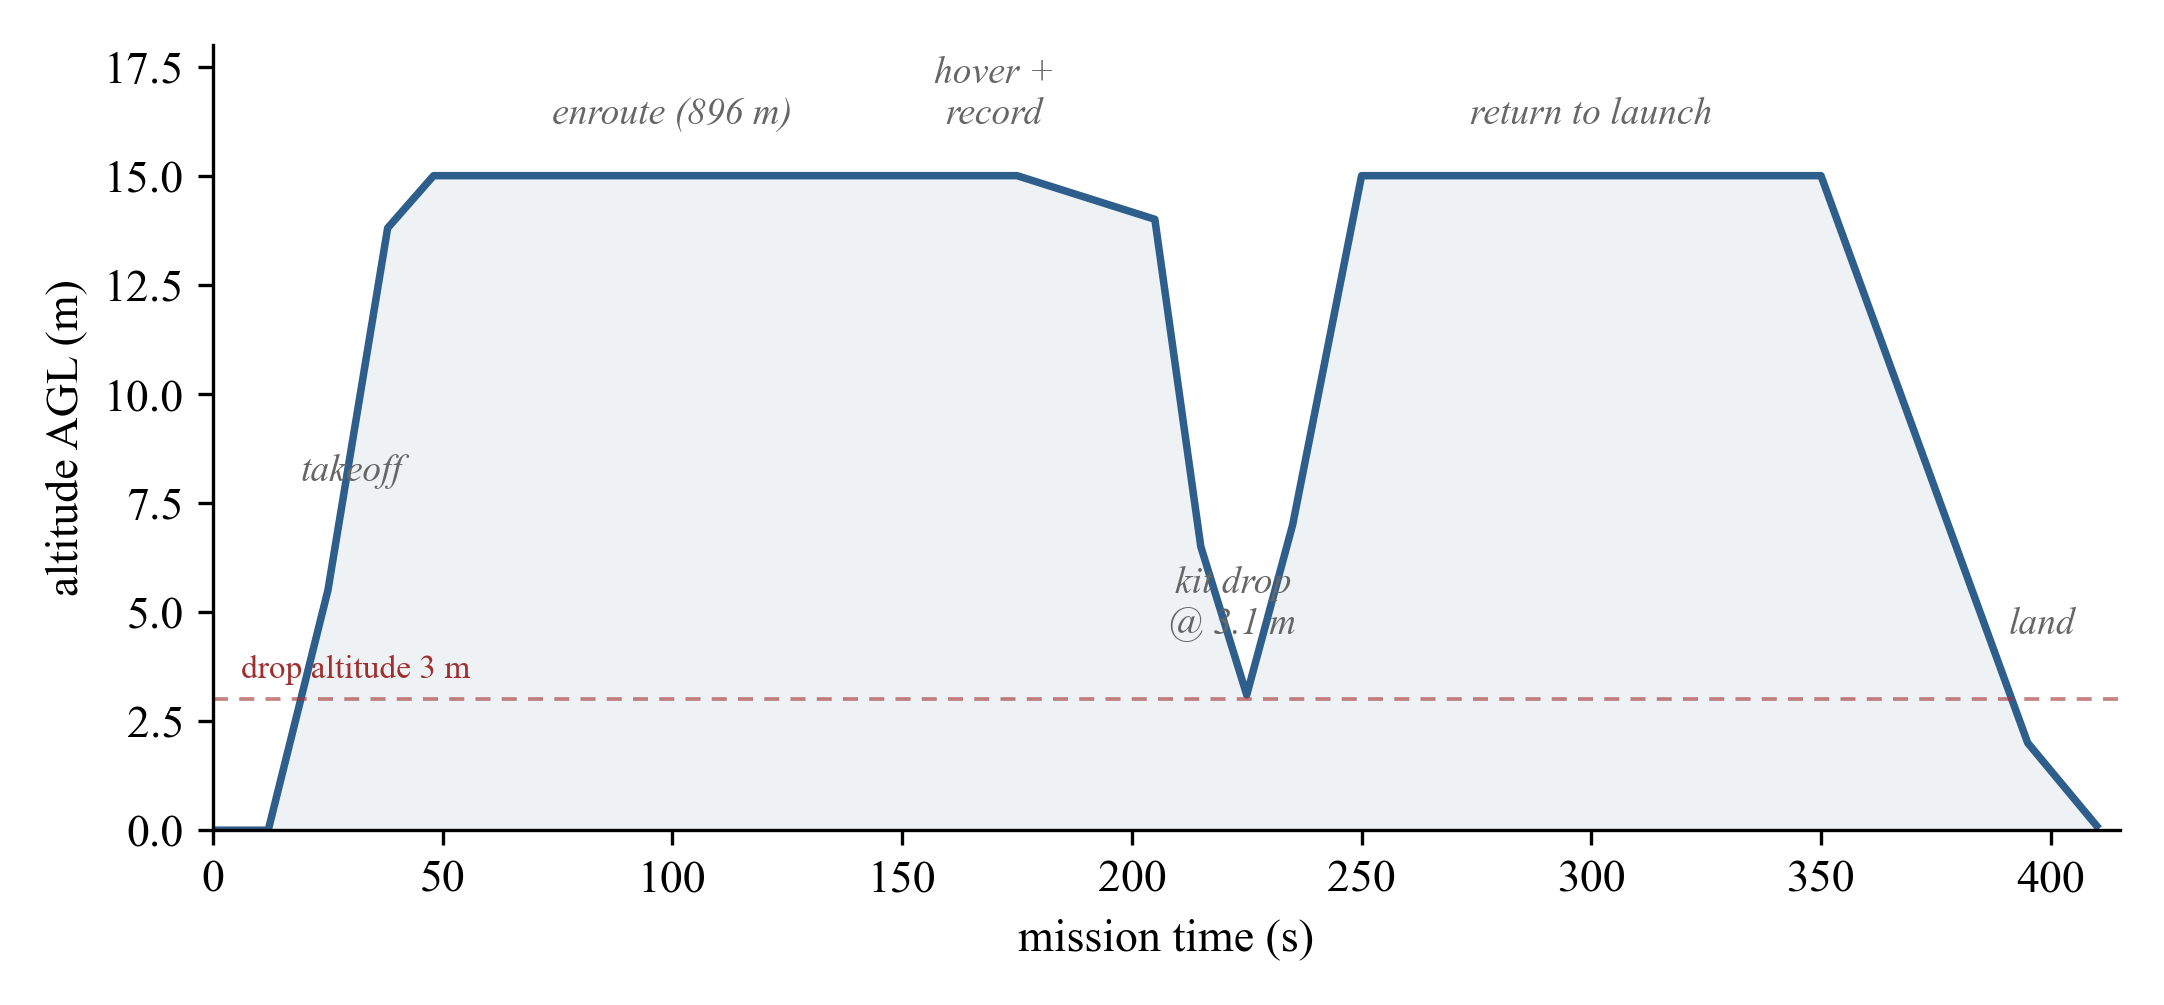
\includegraphics[width=\textwidth]{fig8_mission_profile.png}
\caption{Altitude--time profile of the SITL response mission: takeoff
to 15~m, enroute (896~m), hover + record, descent to the 3~m drop
altitude with kit release commanded at 3.1~m, climb-out, return to
launch, and landing.}
\label{fig:profile}
\end{figure}

Unit tier: \textbf{68/68 pass} on the current implementation.

What this proves --- and only this: the \emph{architecture} is sound
and the \emph{integration} is real. Every interface a hardware phase
will use (packet bytes, clip convention, thresholds, trigger payload,
servo command) was exercised in its production form. What it
deliberately does not prove is acoustic detection performance --- see
\S\ref{sec:notmeasured}.

\section{Defect case studies (retained from v1)}
\label{sec:defects}

Three defects found during v1 are retained as evidence for the design
philosophy, because they now protect the whole VanniKawachh chain.

\textbf{Case 1 --- the silent mode rejection (run 1).} State machine
reached TAKEOFF, altitude stayed 0.0~m, vehicle disarmed itself. Log
forensics showed mode still STABILIZE despite the client reporting
GUIDED. Root cause: unverified setter (H1). Fix:
\S\ref{sec:verifiedmode}. Lesson: \emph{the autopilot's report is the
only truth; the client's state is a wish} --- the same lesson the
two-stage acoustic pipeline applies to Stage-1 claims.

\textbf{Case 2 --- the racing test predicate (run 2).} The harness
inferred ``connected'' from a telemetry state string and raced a
transition. Fix: an explicit boolean on \texttt{/health}. Lesson:
tests must consume \emph{interfaces}, not coincidences of internal
state.

\textbf{Case 3 --- the unguarded abort path (found by review, closed
before it fired).} The original abort used the bare setter --- the
exact call proven unreliable in Case 1 --- and returned with the
vehicle airborne (H2+H3 compound). The unit tier now contains the
regression tests that would have caught both. Lesson: \emph{the
emergency path must be held to a higher standard than the nominal
path, and it is the one most easily left to a lower one.}

\section{What is not yet measured (Phase 1--2 work in progress)}
\label{sec:notmeasured}

Stated plainly, because the credibility of the measured numbers
depends on the honesty of the unmeasured ones:
\begin{itemize}
\item \textbf{No Stage-1 accuracy number exists.} The TFLite-Micro
  model is a hook; training it on scream/cry/keyword data (``help'',
  ``bachao'') and flashing it to the ESP32-S3 is Phase~1. The
  $<$50~ms figure is the design budget for a
  \texttt{micro\_speech}-class model, not a measurement.
\item \textbf{No Stage-2 accuracy number exists for this deployment.}
  The Phase-0 score came from the labelled energy-heuristic
  \emph{fallback}, scoring a \emph{synthesized} clip. PANNs' published
  AudioSet performance~\cite{panns} motivates the backend choice but
  is not a claim about this system's field precision. Phase-1 bench
  work measures Stage-2 latency and end-to-end false-positive rate on
  real street noise, and tunes the fusion weights.
\item \textbf{No radio range or loss figures exist.} LoRa range
  (urban/open) and packet loss vs.\ spreading factor, and ESP-NOW
  clip-delivery reliability, are Phase-2 measurements.
\item \textbf{No hardware flight has occurred.} All flight results are
  SITL (ArduCopter 3.3 --- a 2015 vintage whose command-delivery
  faults usefully forced the defensive design, but a vintage
  nonetheless); Phase~3's staged progression (bench $\rightarrow$
  props-off $\rightarrow$ manual hover $\rightarrow$ guided leg
  $\rightarrow$ full auto, VLOS) governs the transition.
\end{itemize}

These are the numbers the Phase 1--2 bench campaigns exist to produce,
and the papers derived from this thesis will carry them only once
measured.

% ================================================================ Chapter 7
\chapter{Safety, Privacy, and Legal Compliance}
\label{ch:compliance}

\section{Privacy by construction}
\label{sec:privacy}

No continuous recording or transmission exists anywhere in the system,
structurally: audio is processed in-place on the node, frame by frame,
and a frame that does not trip Stage~1 is discarded --- nothing
stored, nothing transmitted. Only event-triggered clips of at most 5~s
ever leave a node, and the accompanying alert is encrypted. The node
cannot stream even if compromised at the configuration level, because
the transport budget (LoRa) cannot carry audio and the clip path is
event-gated in firmware. On the drone, the camera records only over
the incident scene during the hover/delivery window, mission-tagged,
for evidentiary use --- never in transit. This posture is stated
verbatim in the project plan and repeated on every public-facing
description of the system, because a listening-infrastructure project
earns deployment consent with exactly this property.

The same posture is what India's \textbf{Digital Personal Data
Protection Act, 2023}~\cite{dpdp} asks of a deployment. The Act's
data-minimisation and purpose-limitation principles are satisfied
structurally rather than by policy: on-device processing means no
personal data is collected at all for the overwhelming majority of
frames (a discarded frame is never ``processed'' off the node); the
only audio that ever constitutes stored data is the event-triggered
clip of at most 5~s, retained as incident evidence for a lawful
purpose (aid to a person in distress and evidence for law
enforcement); and the encrypted alert carries an event class and
sensor flags, not speech content. A deployed system would still owe
DPDP-compliant notice (signage at instrumented locations), a retention
schedule for clips and mission video, and a designated data fiduciary
--- all deployment-phase obligations noted here so that the
prototype's architecture does not have to change to meet them.

\section{Alert integrity --- why spoofing is closed}
\label{sec:integrity}

An unauthenticated alert channel would make the system an attack tool:
anyone with a Rs.~500 radio could launch a police-alerting drone at
will. Every LoRa packet is therefore sealed (AES-128-CTR
confidentiality, truncated HMAC-SHA256 authenticity, per-node derived
keys, monotonic replay counter --- \S\ref{sec:packetsecurity}); the
hub drops unknown node ids, bad MACs, and stale counters before any
processing. Above the radio layer, the hub reaches the drone stack
through the same token-authenticated, geofence-validated API as any
operator. The residual risks are stated: physical node capture
(mitigated by per-node keys --- one captured node compromises one
pole, revocable in the registry), and radio jamming (a denial, not a
spoof; multi-node corroboration and hub-side node-liveness monitoring
are the future answers).

\section{Flight law (India, Drone Rules 2021)}
\label{sec:flightlaw}

Flight operations are governed by \textbf{The Drone Rules, 2021},
notified by the Ministry of Civil Aviation as \textbf{G.S.R.~589(E)}
on 25 August 2021~\cite{dronerules}. Three of the Rules' mechanisms
bear directly on this project. First, \textbf{registration}: every
drone must be registered on the DigitalSky platform and issued a
Unique Identification Number (UIN); the prototype airframe is
registered accordingly. Second, the \textbf{airspace zoning map}:
DigitalSky publishes an interactive map dividing Indian airspace into
\textbf{green zones} (operations up to 120~m AGL without prior
permission), \textbf{yellow zones} (controlled airspace, prior
permission required), and \textbf{red zones} (operations generally
prohibited); all prototype flying is planned inside a green zone, and
the 120~m altitude bound of the green-zone regime is enforced
software-side at the API edge, with the geofence enforced both at the
edge and in flight. Third, \textbf{operating category}: all prototype
flying is \textbf{VLOS-only}, in an open private field, with an RC
transmitter in a safety pilot's hand as the override authority
(\S\ref{sec:refuses}). Autonomous beyond-visual-line-of-sight response
--- what a deployed VanniKawachh would ultimately perform --- is
described in this thesis strictly as a supervised pilot-program
pathway requiring regulatory engagement under the Rules, not as
something the prototype does. The kit-drop payload is a first-aid kit
released from $\leq 3$~m over the incident point, with the
fail-$\rightarrow$-RTL rule of \S\ref{sec:delivering}; nothing is ever
dropped from transit altitude.

\section{Dispatch restraint}
\label{sec:restraint}

The system's authority to launch an aircraft is gated three times:
Stage-1 detection (recall-tuned, on the node), Stage-2 verification
plus fused severity against explicit thresholds (precision-tuned, on
the hub, pinned by tests asserting no dispatch below threshold), and
the flight stack's own edge validation and queue admission. Every
held-back incident is still logged and dashboard-visible --- restraint
in dispatch is not silence toward the police.

\section{Radio-spectrum compliance}
\label{sec:spectrum}

The LoRa alert link must itself be lawful. In India, spectrum use is
administered by the \textbf{Wireless Planning and Coordination (WPC)
Wing} of the Department of Telecommunications, which has
\textbf{delicensed the 865--867~MHz band} for low-power wireless
devices~\cite{wpc} --- the band in which Indian LoRaWAN deployments
ordinarily operate without an operator licence, subject to the
notified power and bandwidth limits. The SX1278 modules used in the
prototype are 433~MHz parts; 433~MHz operation in India falls under
the WPC's separate \textbf{low-power short-range device (SRD)
provisions}, which permit only very low radiated power. The
prototype's bench and field-test configuration therefore respects the
applicable low-power limits, and the deployment plan standardizes on
\textbf{865--867~MHz} hardware (SX1276-class radios) for any at-scale
installation, where the delicensed band offers both legal headroom and
better link budget at permitted power. This is a procurement change,
not a design change: the packet format, cryptography, and gateway
software of Chapter~\ref{ch:node-hub} are frequency-agnostic.

% ================================================================ Chapter 8
\chapter{Conclusions and Future Work}
\label{ch:conclusion}

\section{Conclusions}
\label{sec:conclusions}

VanniKawachh demonstrates that the components of an
infrastructure-borne women-safety chain --- TinyML screening on a
solar pole budget, pretrained deep audio verification on a locality
hub, sealed alerting over an operator-free radio, and a
safety-interlocked autonomous first response --- integrate into a
single system whose architecture can be proven end-to-end in
simulation before any hardware is soldered. The project's governing
discipline, inherited from the v1 flight stack and extended to every
new layer, is that \emph{a claim is not a confirmation}: a Stage-1 hit
is not an incident until Stage~2 and fusion say so; a packet is not an
alert until its MAC and counter say so; a mode command is not a mode
until the autopilot's telemetry says so; a ``finished'' mission is not
finished until the vehicle is disarmed on the ground. Under that
discipline the full-chain rehearsal passed on the first architecture
(fused severity 0.88, kit release at 3.1~m, 328~s mission, 8/8
acceptance checks, 68/68 unit cases), and the remaining work is
measurement and hardening, not redesign.

Equally deliberate is what this thesis does not claim: no acoustic
accuracy has been asserted that was not measured, and every number
produced by a stand-in is labelled. The literature's 97.5\%-accurate
wearables fail when absent; a system that aspires to replace them must
not begin life with numbers that fail when examined.

\section{Future work}
\label{sec:futurework}

\begin{enumerate}
\item \textbf{Phase 1--2 measurement campaigns} --- train and flash
  the Stage-1 TFLM model; measure outdoor detection distance vs.\ SNR,
  Stage-1 and Stage-2 latency, end-to-end false-positive rate on
  street noise; measure LoRa range and loss vs.\ spreading factor;
  tune the fusion weights against bench data.
\item \textbf{Live police streaming} --- RTSP/WebRTC video from the
  drone to the dashboard over LTE, extending the evidence recorder of
  \S\ref{sec:camera} into a real-time feed for responding officers.
\item \textbf{OpenCV victim tracking} --- on-drone detection and
  framing of the person in distress during hover, keeping the camera
  and the aircraft usefully positioned without operator input.
\item \textbf{TDOA multi-node localization} --- with synchronized
  clocks, time-difference-of-arrival across neighbouring nodes
  upgrades ``which pole heard it'' to a position estimate between
  poles, and provides the multi-node corroboration path sketched in
  \S\ref{sec:rationale}.
\item \textbf{City-scale mesh} --- many nodes per hub, many hubs per
  city; hub-to-hub LoRa or wired backhaul; fleet dispatch with
  per-airframe interlocks (the v1 multi-vehicle design carries over).
\item \textbf{Flight-stack modernization} (inherited from v1) ---
  pymavlink~\cite{pymavlink} / MAVSDK migration, ArduPilot 4.x SITL
  validation, fault-injection flight campaigns, and the Phase-3/4
  hardware progression flown on the documented build.
\end{enumerate}

% ================================================================ references
\begin{thebibliography}{34}

\bibitem{pavithra}
R.~Pavithra, R.~Ahalya, and C.~Shuruthika, ``Discreet AI-powered
women's safety app with audio recognition and emergency automation,''
in \emph{Proc.\ 2026 IEEE Students Conf.\ Eng.\ Syst.\ (SCEECS)},
Bhopal, India, 2026, doi: 10.1109/SCEECS68810.2026.11430037.

\bibitem{kimwindow}
Y.~Kim, D.~Jang, and S.-P.~Lee, ``Robust scream detection and scream
temporal interval prediction using CNN-Transformer and windowing
CNN,'' \emph{IEEE Access}, vol.~13, pp.~71374--71387, 2025, doi:
10.1109/ACCESS.2025.3556729.

\bibitem{sharma}
P.~Sharma and T.~J.~Jebaseeli, ``Smart scream and panic detection
system for women using AI,'' in \emph{Proc.\ 2025 Int.\ Conf.\ Autom.\
Comput.\ Renew.\ Syst.\ (ICACRS)}, 2025, pp.~1554--1559, doi:
10.1109/ICACRS67045.2025.11324333.

\bibitem{srimathi}
A.~Srimathi, S.~Jothi, and M.~P.~Sindhiya, ``Human scream detection
and analysis for crime reduction,'' in \emph{Proc.\ 2025 Int.\ Conf.\
Multidiscip.\ Sci.\ Comput.\ Intell.\ (ICMSCI)}, Erode, India, 2025,
pp.~1528--1534, doi: 10.1109/ICMSCI62561.2025.10894058.

\bibitem{bharathi}
P.~S.~Bharathi et al., ``A novel IoT enabled women safety system
design with emergency alert mechanism,'' in \emph{Proc.\ 2025 Int.\
Conf.\ Future Technol.\ Syst.\ (ICFTS)}, 2025, pp.~1--7, doi:
10.1109/ICFTS62006.2025.11031774.

\bibitem{snehith}
R.~Snehith, S.~Saranya, and N.~R.~Reddy, ``A smart device for women
safety using IoT,'' in \emph{Proc.\ 2025 Int.\ Conf.\ Intell.\ Syst.\
Sci.\ (ICISS)}, 2025, pp.~277--282, doi:
10.1109/ICISS63372.2025.11076270.

\bibitem{kimscream}
Y.~Kim, D.~Jang, and J.~Lee, ``Development of scream detection system
with large-scale scream dataset,'' in \emph{Proc.\ 2024 Int.\ Conf.\
Inf.\ Commun.\ Technol.\ Converg.\ (ICTC)}, Jeju, South Korea, 2024,
pp.~590--593, doi: 10.1109/ICTC62082.2024.10826757.

\bibitem{fime}
A.~A.~Fime, M.~Ashikuzzaman, and A.~Aziz, ``Audio signal-based danger
detection using signal processing and deep learning,'' \emph{Expert
Systems with Applications}, vol.~237, art.\ no.~121646, Mar.\ 2024,
doi: 10.1016/j.eswa.2023.121646.

\bibitem{hadkar}
R.~V.~Hadkar et al., ``An efficient IoT-enabled women safety device,''
in \emph{Proc.\ 2024 Int.\ Conf.\ Autom.\ Comput.\ Renew.\ Syst.\
(ICACRS)}, 2024, pp.~425--431, doi:
10.1109/ICACRS62842.2024.10841797.

\bibitem{uganya}
G.~Uganya et al., ``Smart women safety device using IoT and GPS
tracker,'' in \emph{Proc.\ 2023 Int.\ Conf.\ Comput.\ Electron.\
Biomed.\ Syst.\ (ICCEBS)}, Chennai, India, 2023, pp.~1--6, doi:
10.1109/ICCEBS58601.2023.10449302.

\bibitem{potturi}
S.~Potturi et al., ``An SOS women safety device: Automatic emergency
alerts and geo-location sharing with GSM/GPS integration,'' in
\emph{Proc.\ 2026 Int.\ Conf.\ Intell.\ Comput.\ Netw.\ Syst.\
(IC-ICNS)}, Bhubaneswar, India, 2026, pp.~1--6, doi:
10.1109/IC-ICNS68863.2026.11537940.

\bibitem{ciaburro}
G.~Ciaburro and V.~Puyana-Romero, ``Sound event detection in smart
cities: A systematic review of methods, datasets, and applications,''
\emph{Big Data and Cognitive Computing}, vol.~10, no.~3, art.\
no.~83, 2026, doi: 10.3390/bdcc10030083.

\bibitem{panns}
Q.~Kong, Y.~Cao, T.~Iqbal, Y.~Wang, W.~Wang, and M.~D.~Plumbley,
``PANNs: Large-scale pretrained audio neural networks for audio
pattern recognition,'' \emph{IEEE/ACM Trans.\ Audio, Speech, Lang.\
Process.}, vol.~28, pp.~2880--2894, 2020, doi:
10.1109/TASLP.2020.3030497; \texttt{panns-inference} package.

\bibitem{tflm}
R.~David et al., ``TensorFlow Lite Micro: Embedded machine learning
for TinyML systems,'' in \emph{Proc.\ Mach.\ Learn.\ Syst.\ (MLSys)},
vol.~3, 2021, pp.~800--811; documentation and the
\texttt{micro\_speech} example,
\url{https://www.tensorflow.org/lite/microcontrollers}.

\bibitem{ardupilot}
ArduPilot Development Team, ``ArduPilot documentation'' (firmware,
SITL, and failsafe documentation), \url{https://ardupilot.org}; and
MAVLink Development Team, ``MAVLink developer guide'' (HEARTBEAT,
SET\_MODE, COMMAND\_LONG/MAV\_CMD\_DO\_SET\_MODE,
MAV\_CMD\_DO\_SET\_SERVO), \url{https://mavlink.io/en/}. Accessed
Jul.\ 2026.

\bibitem{lorawan}
LoRa Alliance, ``LoRaWAN L2 1.0.4 specification,'' LoRa Alliance
Technical Committee, 2020. [Online]. Available:
\url{https://lora-alliance.org/resource_hub/lorawan-104-specification-package/}.

\bibitem{fips197}
National Institute of Standards and Technology, ``Advanced Encryption
Standard (AES),'' FIPS PUB 197, Nov.\ 2001, doi:
10.6028/NIST.FIPS.197.

\bibitem{rfc2104}
H.~Krawczyk, M.~Bellare, and R.~Canetti, ``HMAC: Keyed-hashing for
message authentication,'' IETF RFC 2104, Feb.\ 1997.

\bibitem{dronerules}
Ministry of Civil Aviation, Government of India, ``The Drone Rules,
2021,'' notification G.S.R.~589(E), \emph{Gazette of India}, 25 Aug.\
2021; DigitalSky platform (UIN registration and airspace zone map).
\url{https://digitalsky.dgca.gov.in}. Accessed 2026-07-06.

\bibitem{dpdp}
Government of India, ``The Digital Personal Data Protection Act,
2023,'' Act No.~22 of 2023, \emph{Gazette of India}, 11 Aug.\ 2023.

\bibitem{wpc}
Wireless Planning and Coordination Wing, Department of
Telecommunications, Government of India --- delicensing of the
865--867~MHz band for low-power wireless devices (G.S.R.~1048(E),
2005) and low-power short-range-device (SRD) provisions applicable to
433~MHz operation.

\bibitem{dronekit}
DroneKit-Python 2.9.2.
\url{https://github.com/dronekit/dronekit-python}. Accessed
2026-07-06.

\bibitem{pymavlink}
pymavlink. \url{https://github.com/ArduPilot/pymavlink}. Accessed
2026-07-06.

\bibitem{dronekitsitl}
dronekit-sitl 3.3.0. \url{https://github.com/dronekit/dronekit-sitl}.
Accessed 2026-07-06.

\bibitem{fastapi}
FastAPI. \url{https://fastapi.tiangolo.com}. Accessed 2026-07-06.

\bibitem{react}
React 18. \url{https://react.dev}. Accessed 2026-07-06.

\bibitem{leaflet}
Leaflet 1.9. \url{https://leafletjs.com}. Accessed 2026-07-06.

\bibitem{osm}
OpenStreetMap. \url{https://www.openstreetmap.org}. Accessed
2026-07-06.

\bibitem{pixhawk}
Pixhawk hardware reference. \url{https://pixhawk.org}. Accessed
2026-07-06.

\bibitem{rpi5}
Raspberry Pi 5 product documentation.
\url{https://www.raspberrypi.com/documentation/}. Accessed 2026-07-06.

\bibitem{esp32s3}
Espressif ESP32-S3 technical reference manual.
\url{https://www.espressif.com}. Accessed 2026-07-06.

\bibitem{sx1278}
Semtech SX1276/77/78/79 LoRa transceiver datasheet.
\url{https://www.semtech.com}. Accessed 2026-07-06.

\bibitem{inmp441}
InvenSense/TDK INMP441 omnidirectional I2S MEMS microphone datasheet.
\url{https://invensense.tdk.com}. Accessed 2026-07-06.

\bibitem{faa107}
U.S. FAA, Part 107 --- Small Unmanned Aircraft Systems.
\url{https://www.faa.gov/uas/commercial_operators}. Accessed
2026-07-06.

\end{thebibliography}

% ================================================================ appendices
\appendix

\chapter{LoRa Alert Packet Wire Format}
\label{app:packet}

25 bytes total --- comfortably one LoRa frame
(Table~\ref{tab:wireformat}).

\begin{table}[htbp]
\centering
\caption{Sealed alert packet wire format (25 bytes).}
\label{tab:wireformat}
\small
\begin{tabular}{@{}ccp{0.62\textwidth}@{}}
\toprule
\textbf{Offset} & \textbf{Size} & \textbf{Field} \\
\midrule
0 & 2 & magic \texttt{"VK"} \\
2 & 1 & version (1) \\
3 & 2 & node\_id (uint16 BE) --- cleartext (selects the key) \\
5 & 4 & counter (uint32 BE) --- cleartext (CTR nonce + replay) \\
9 & 8 & AES-128-CTR ciphertext of payload \\
17 & 8 & MAC: HMAC-SHA256(node\_key, header + ciphertext)[:8] \\
\bottomrule
\end{tabular}
\end{table}

Payload (before encryption): event uint8 (1 = scream,
2 = help\_keyword, 3 = cry, 4 = crash); confidence uint8 (Stage-1,
0--255); PIR uint8 (0/1); light uint8 (LDR 0--255, 0 = dark); battery
uint8 (\%); 3 reserved bytes.

Per-node key = HMAC-SHA256(master\_key, \texttt{"node:<id>"})[:16].
Rejection rules at the hub: bad length, bad magic/version, bad MAC,
unknown node\_id, counter $\leq$ last accepted.

\chapter{Configuration Reference}
\label{app:config}

\begin{table}[htbp]
\centering
\caption{Hub configuration (\texttt{hub/config.py}).}
\label{tab:hubconfig}
\small
\begin{tabular}{@{}p{0.32\textwidth}p{0.22\textwidth}p{0.34\textwidth}@{}}
\toprule
\textbf{Variable} & \textbf{Default} & \textbf{Governs} \\
\midrule
\texttt{HUB\_MASTER\_KEY} & dev key (must be set in deployment) &
AES-128 master key (hex) \\
\texttt{VERIFY\_THRESHOLD} & 0.50 & Min Stage-2 audio score to count
as distress \\
\texttt{DISPATCH\_THRESHOLD} & 0.60 & Min fused severity to launch
the drone \\
\texttt{CLIP\_WAIT\_S} & 8.0 & Wait for the WiFi clip before degraded
scoring \\
\texttt{GATEWAY\_PORT} / \texttt{GATEWAY\_BAUD} & COM3 / 115200 &
Gateway ESP32 serial \\
\texttt{DRONE\_API\_URL} / \texttt{DRONE\_API\_TOKEN} &
localhost:8000 / unset & Drone stack endpoint \\
\texttt{NODES\_FILE} / \texttt{CLIPS\_DIR} & \texttt{hub/nodes.json}
/ \texttt{hub/clips} & Registry and clip storage \\
\texttt{CLIP\_SERVER\_PORT} & 8990 & Node clip upload server \\
\bottomrule
\end{tabular}
\end{table}

\begin{table}[htbp]
\centering
\caption{Flight-stack configuration (\texttt{flight\_core/config.py},
v2 additions).}
\label{tab:flightconfig}
\small
\begin{tabular}{@{}p{0.36\textwidth}p{0.24\textwidth}p{0.28\textwidth}@{}}
\toprule
\textbf{Variable} & \textbf{Default} & \textbf{Governs} \\
\midrule
\texttt{PAYLOAD\_SERVO\_CHANNEL} & 9 (Pixhawk AUX OUT 1) & Kit-release
servo output \\
\texttt{PAYLOAD\_OPEN\_PWM} / \texttt{PAYLOAD\_HOLD\_PWM} & 1900 /
1100 & Hook open / closed \\
\texttt{PAYLOAD\_DROP\_ALT} & 3.0~m & Descend-to altitude before
release \\
\bottomrule
\end{tabular}
\end{table}

The full v1 flight-stack configuration table (connection string, home,
geofence, battery thresholds, GPS debounce, stall timeout, queue
bounds, API token, \texttt{SITL\_MODE}) is unchanged and lives in
\texttt{docs/SYSTEM\_DOCUMENTATION.md} \S 7.

\chapter{Test Inventory}
\label{app:tests}

\textbf{Tier 1 --- 68 collected cases.}
\texttt{tests/test\_units.py} (47): 10 failsafe-arbiter cases
(thresholds, escalation, no-downgrade, debounce $\times 2$, fire-once,
geofence, timeout, healthy baseline); 7 queue cases (priority, depth
cap, prune, cancel $\times 3$, worker bookkeeping); 2 persistence
cases; validation cases covering every rejection bound (coordinates,
altitude, hover, priority, waypoints --- including parametrized edge
values); 3 configuration cases.
\texttt{tests/test\_hub.py} (14): packet seal/unseal round-trip; MAC
tamper rejection; replay-counter rejection; registry lookup +
unknown-node drop; fusion scoring and priority mapping; pipeline
gating (no dispatch below verify/dispatch thresholds); degraded
no-clip scoring; dispatcher payload shape.
\texttt{tests/test\_obstacle\_avoidance.py} (7): keep-out routing
geometry.

\textbf{Tier 2 --- \texttt{tests/test\_full\_mission.py}:} the
eight-property SITL acceptance flight of \S\ref{sec:methodology},
runnable on any machine.

\textbf{Tier 3 --- \texttt{scripts/demo\_phase0.py}:} the
zero-hardware full-chain rehearsal of \S\ref{sec:phase0results}
(sensing sim $\rightarrow$ hub $\rightarrow$ SITL flight $\rightarrow$
kit drop), exit 0 on a completed mission.

\end{document}
